\documentclass[a4paper,11pt,oneside,openany]{report}

\usepackage[utf8]{inputenc}
\usepackage[T1]{fontenc}
\usepackage{lmodern}
\usepackage[a4paper,top=3cm,bottom=3cm,left=3cm,right=3cm]{geometry}
\usepackage{helvet}
\usepackage[english]{babel}
\usepackage{csquotes}
\usepackage[backend=biber,style=numeric,sorting=none]{biblatex}
\usepackage{parskip}
\usepackage[margin=1cm]{caption}
\usepackage{booktabs}
\usepackage{array}
\usepackage{longtable}
\usepackage{tabularx}
\usepackage{amsmath}
\usepackage{amssymb}
\usepackage{enumitem}
\usepackage{graphicx}
\usepackage{float}
\usepackage{xcolor}
\usepackage{microtype}
\usepackage{setspace}
\usepackage{titlesec}
\usepackage{hyperref}
\ifdefined\pdfadjustspacing
  \pdfadjustspacing=1
\fi

\newcolumntype{L}[1]{>{\raggedright\arraybackslash}p{#1}}
\newcolumntype{Y}{>{\raggedright\arraybackslash}X}

\definecolor{thesisblue}{HTML}{1F4E79}
\definecolor{thesisaccent}{HTML}{B8651B}
\definecolor{thesisgray}{HTML}{F3F5F7}
\definecolor{thesisline}{HTML}{D7DEE6}

\newcommand{\mylastname}{Bakkoury}
\newcommand{\myfirstname}{Anas}
\newcommand{\mynumber}{30007440}
\newcommand{\myname}{\myfirstname{} \mylastname{}}
\newcommand{\mytitle}{Prompt Decomposition Strategies for Reliable Telematics-Based Fleet Monitoring Using Llama3 and DeepSeek}
\newcommand{\mysupervisor}{Prof. Dr.-Ing. Hendro Wicaksono}
\newcommand{\mysubmissiondate}{12 May 2026}
\newcommand{\constructorlogopath}{figures/constructor_logo.jpeg}
\newcommand{\metric}[1]{\texttt{\detokenize{#1}}}
\newcommand{\strategy}[1]{\texttt{\detokenize{#1}}}
\newcommand{\summarynote}[2]{%
  \par\smallskip
  \noindent\begingroup
  \setlength{\fboxsep}{7pt}%
  \colorbox{thesisgray}{%
    \parbox{\dimexpr\linewidth-2\fboxsep\relax}{%
      \small\textbf{#1.} #2%
    }%
  }%
  \endgroup\par\smallskip
}

\newcommand{\thesislogo}{%
  \IfFileExists{\constructorlogopath}{%
    \includegraphics[width=0.36\textwidth]{\constructorlogopath}%
  }{\vspace*{18mm}}%
}

\hypersetup{
  pdfauthor = {\myname},
  pdftitle = {\mytitle},
  pdfkeywords = {large language models, prompt decomposition, telematics analytics, graph recovery, fleet monitoring, causal relationship extraction},
  colorlinks = true,
  linkcolor = thesisblue,
  citecolor = thesisblue,
  urlcolor = thesisblue
}

\captionsetup{font=small,labelfont=bf,justification=raggedright,singlelinecheck=false,skip=6pt}
\setstretch{1.08}
\setlength{\emergencystretch}{2em}
\hyphenation{intelligence governance artifacts decomposition prompting behaviour telematics}
\setlength{\textfloatsep}{16pt plus 3pt minus 3pt}
\setlength{\floatsep}{14pt plus 3pt minus 3pt}
\setlength{\intextsep}{14pt plus 3pt minus 3pt}
\renewcommand{\arraystretch}{1.12}
\clubpenalty=10000
\widowpenalty=10000
\displaywidowpenalty=10000
\raggedbottom
\setlist[itemize]{leftmargin=*,nosep}
\setlist[enumerate]{leftmargin=*,nosep}
\titleformat{\chapter}[display]
  {\normalfont\sffamily\huge\bfseries}
  {\color{thesisblue}\Large\chaptertitlename\ \thechapter}
  {0.4ex}
  {\titlerule[0.8pt]\vspace{1.2ex}}
  [\vspace{0.8ex}\titlerule]
\titlespacing*{\chapter}{0pt}{-12pt}{24pt}
\titleformat{\section}
  {\normalfont\sffamily\Large\bfseries}
  {\thesection}
  {0.8em}
  {}
\titleformat{\subsection}
  {\normalfont\sffamily\large\bfseries}
  {\thesubsection}
  {0.75em}
  {}
\titleformat{\subsubsection}
  {\normalfont\sffamily\normalsize\bfseries}
  {\thesubsubsection}
  {0.7em}
  {}
\titlespacing*{\section}{0pt}{2.6ex plus 0.8ex minus 0.2ex}{1.2ex}
\titlespacing*{\subsection}{0pt}{2.0ex plus 0.6ex minus 0.2ex}{0.8ex}
\titlespacing*{\subsubsection}{0pt}{1.4ex plus 0.5ex minus 0.2ex}{0.6ex}
\setcounter{tocdepth}{2}
\setcounter{secnumdepth}{3}

\addbibresource{references.bib}

\begin{document}
  \pagenumbering{gobble}

  \begin{titlepage}
    \thispagestyle{empty}
    \centering

    \vspace*{8mm}
    \thesislogo

    \vspace*{34mm}
    {\setstretch{1.12}\LARGE\bfseries \mytitle\par}

    \vspace*{12mm}
    {\large Bachelor Thesis\par}
    \vspace*{1.5mm}
    {\large Computer Science\par}

    \vfill

    \begin{tabular}{@{}>{\bfseries}L{38mm}L{78mm}@{}}
      Author & \myname \\
      Supervisor & \mysupervisor \\
      Submission date & \mysubmissiondate \\
    \end{tabular}

    \vspace*{24mm}
    {\small Constructor University\par}
    \vspace*{1mm}
    {\small School of Computer Science and Engineering\par}
  \end{titlepage}

  \pagenumbering{roman}
  \thispagestyle{empty}

  \chapter*{Statutory Declaration}
  \addcontentsline{toc}{chapter}{Statutory Declaration}

  \begin{center}
    \begin{tabular}{|L{45mm}|L{85mm}|}
      \hline
      Family Name, Given/First Name & \mylastname, \myfirstname \\
      Matriculation number & \mynumber \\
      Kind of thesis submitted & Bachelor Thesis \\
      \hline
    \end{tabular}
    \vspace*{8mm}
  \end{center}

  \subsection*{English: Declaration of Authorship}

  I hereby declare that this thesis was created and written solely by myself
  without unauthorized external support. Any sources, direct or indirect, are
  marked as such. I am aware that the thesis in digital form may be reviewed
  for unauthorized aid and plagiarism. This document has not been submitted to
  another examination board and has not been published.

  \subsection*{German: Erklaerung der Autorenschaft}

  Ich erklaere hiermit, dass die vorliegende Arbeit ohne unzulaessige fremde
  Hilfe ausschliesslich von mir erstellt und geschrieben worden ist. Alle
  verwendeten Quellen, direkter oder indirekter Art, sind als solche kenntlich
  gemacht. Diese Arbeit wurde keiner anderen Pruefungsbehoerde vorgelegt und
  bisher nicht veroeffentlicht.

  \vspace{20mm}

  \dotfill\\
  Date, Signature

  \newpage

  \chapter*{Declaration on the Use of Artificial\\ Intelligence Tools}
  \addcontentsline{toc}{chapter}{Declaration on the Use of Artificial Intelligence Tools}

  I hereby declare that artificial intelligence (AI) tools were used during the
  preparation of this thesis in a limited and transparent supporting role.
  Their use was confined to language refinement, code-related assistance,
  debugging support, and workflow improvements. All AI-assisted outputs were
  critically reviewed, verified, and edited by me to ensure correctness,
  academic integrity, and alignment with the objectives of this research.

  The research design, experimental setup, analysis, interpretation of results,
  and conclusions presented in this thesis are my own intellectual
  contributions.

  \begin{table}[H]
    \centering
    \caption*{AI tools used during thesis preparation}
    \label{tab:ai_tools_declaration}
    \begin{tabularx}{\textwidth}{@{}L{0.27\textwidth}Y@{}}
      \toprule
      \textbf{AI Tool} & \textbf{Purpose of Use} \\
      \midrule
      ChatGPT 5.5 &
      Used to support language refinement, grammar improvement, academic
      phrasing, structural feedback, and clarification of technical
      explanations. \\
      Grammarly Pro &
      Used for grammar checking, spelling correction, punctuation improvement,
      and readability enhancement. \\
      DeepL Translator &
      Used for limited translation support and language refinement between
      English and German where necessary. \\
      Claude Sonnet 4.6 &
      Used to support implementation work, code refinement, debugging
      suggestions, and software engineering workflow improvements. \\
      \bottomrule
    \end{tabularx}
  \end{table}

  No AI system was used to fabricate experimental results, falsify data,
  generate unverified findings, or produce conclusions presented as original
  scientific contributions without human verification.

  I take full responsibility for the accuracy, integrity, and originality of all
  content contained in this thesis.

  \newpage

  \chapter*{Abstract}
  \addcontentsline{toc}{chapter}{Abstract}

  Fleet monitoring increasingly depends on vehicle telemetry whose meaning is
  relational rather than purely descriptive: energy state, speed,
  acceleration, mileage, and distance become operationally useful when their
  directed dependencies are made explicit. This thesis evaluates whether local
  open-source large language models can support this task by proposing
  directed feature graphs from a normalized Tesla electric-vehicle telemetry
  dataset.

  The study treats prompt decomposition as the central experimental variable.
  Five strategies are compared: zero-shot prompting, a no-instruction control,
  policy-first structured prompting, least-to-most decomposition, and
  skeleton-of-thought prompting. Two local Ollama models,
  \texttt{llama3.1:8b} and \texttt{deepseek-r1:8b}, generate edge lists over
  six features: \texttt{electricenergyremaining},
  \texttt{electricremaining}, \texttt{speed\_kmh},
  \texttt{acceleration\_kmh2}, \texttt{mileage}, and \texttt{distance\_m}.
  Each output is parsed into a binary adjacency matrix and evaluated against a
  six-edge Tesla energy-consumption ground-truth DAG using precision, recall,
  F1 score, structural Hamming distance, false discovery rate, Pearson
  correlation, Hamming distance, and Frobenius norm.

  The strongest observed model-strategy cell is \texttt{deepseek-r1:8b} with
  \texttt{Strategy\_26} (Skeleton-of-Thought), achieving precision
  \(0.4444\), recall \(0.6667\), F1 score \(0.5333\), structural Hamming
  distance \(7\), and Pearson correlation \(0.4303\). The next-best F1 score
  is \(0.4000\), observed for \texttt{llama3.1:8b} with zero-shot prompting
  and for \texttt{deepseek-r1:8b} with the no-instruction control. The results
  are descriptive because each validated model-strategy cell contains one
  output. They do not establish formal causal discovery, statistical
  significance, or repeated-run self-consistency. Within that evidence, the
  thesis shows that decomposition-style prompting can improve LLM-assisted
  graph recovery in a controlled Tesla EV setting, while still requiring
  explicit safeguards against false positives and direction errors.

  \newpage
  \tableofcontents

  \clearpage
  \pagenumbering{arabic}

  \chapter{Introduction}
\label{sec:introduction}

\section{Problem and Motivation}

Modern fleet monitoring depends on telemetry streams that describe vehicle
state, motion, energy availability, and accumulated usage. In electric
vehicles, measurements such as remaining energy, remaining range proxy, speed,
acceleration, mileage, and travelled distance are not independent facts. Their
operational meaning depends on how they relate: acceleration changes speed,
speed contributes to distance, driving behaviour affects energy consumption,
and remaining energy constrains how a vehicle can be interpreted in a fleet
context.

This relational structure makes graph-based telemetry analysis attractive. A
directed graph can encode proposed dependencies between telemetry features,
while an adjacency matrix makes those dependencies measurable and comparable.
Such representations can support inspection, diagnostics, knowledge-graph
construction, and downstream decision support. They are also difficult to
obtain automatically. Classical causal discovery requires assumptions about
data-generating processes, sufficient observations, and domain validation.
Manual graph construction by experts is more interpretable, but it is costly
and does not scale easily across vehicle systems, datasets, and use cases.

Large language models (LLMs) offer a different kind of support. Rather than
estimating a causal model directly from raw data, an LLM can be asked to
propose a compact directed graph from feature descriptions, domain semantics,
and a statistical fingerprint of the dataset. This should not be confused with
formal causal discovery. In this thesis, the LLM is used as a graph proposal
component: it emits candidate directed edges, the system parses those edges
into an adjacency matrix, and the result is evaluated against an explicit
ground-truth DAG. The scientific question is whether prompt design makes this
proposal process more reliable.

Prompt design is a meaningful research variable because graph recovery
requires more than naming related variables. A model must distinguish direct
from mediated relations, avoid bidirectional or transitive edges unless they
are justified, respect the allowed feature vocabulary, and output a
machine-parseable edge list. Unstructured prompts may produce plausible
correlations, reversed directions, prose explanations, or extra variables.
Structured prompts and prompt decomposition can instead make the model attend
to physical directness, subsystem grouping, and final output constraints.

In this thesis, \emph{prompt decomposition} refers to strategies that divide
the graph-recovery task into smaller internal stages before the final edge
list is produced. The decomposition-oriented strategies are
\texttt{Strategy\_25} (Least-to-Most) and \texttt{Strategy\_26}
(Skeleton-of-Thought). They are compared with \texttt{Strategy\_1}
(Zero-Shot Prompting), \texttt{Strategy\_23} (No-Instruction Control), and
\texttt{Strategy\_24} (Policy-First Structured).

The empirical setting is deliberately focused. The primary evidence is a Tesla
EV result set for two local Ollama models, \texttt{llama3.1:8b} and
\texttt{deepseek-r1:8b}, evaluated on a six-feature energy-consumption
graph-recovery task. This scope makes the work relevant to locally deployed
and infrastructure-constrained fleet analytics, while keeping the claims
auditable. The thesis does not treat the models as inferring true causality
from telemetry alone; it evaluates whether their prompted graph proposals agree
with a predefined physics-informed reference graph.

\section{Research Objective}

The main research question is:

\begin{quote}
To what extent do prompt decomposition and structured prompting strategies
improve LLM-assisted graph recovery from vehicle telematics data when compared
with simpler prompting baselines?
\end{quote}

The question is evaluated in a supervised graph-recovery setting. A predicted
edge set is parsed from each LLM output, converted into an adjacency matrix,
and compared with a fixed Tesla EV ground-truth matrix. The work does not
evaluate formal causal identification, repeated-run self-consistency, or
statistical significance across repeated generations.

The thesis addresses five research questions:

\begin{enumerate}
  \item \textbf{RQ1:} How accurately can \texttt{llama3.1:8b} and
  \texttt{deepseek-r1:8b} recover directed relationships between Tesla EV
  telematics features from a structured dataset summary?

  \item \textbf{RQ2:} How do prompt decomposition strategies, especially
  least-to-most prompting and skeleton-of-thought prompting, compare with
  zero-shot and no-instruction baselines on graph-recovery metrics?

  \item \textbf{RQ3:} How does explicit instruction structuring through a
  policy-first prompt affect precision, recall, false discovery rate, and
  structural graph error?

  \item \textbf{RQ4:} Which evaluated model-strategy combination achieves the
  strongest adjacency-matrix recovery against the Tesla EV ground truth?

  \item \textbf{RQ5:} Which correct, spurious, or reversed relationships
  appear repeatedly across model-strategy outputs, and what do they reveal
  about LLM failure modes in telematics graph recovery?
\end{enumerate}

\section{Contribution Statement}

The thesis makes four contributions:

\begin{itemize}
  \item it defines a reproducible Tesla EV graph-recovery task in which LLM
  outputs are converted into directed adjacency matrices and evaluated against
  a fixed ground-truth DAG;

  \item it compares five prompting strategies across two local open-source
  LLMs, with particular attention to prompt decomposition through
  least-to-most reasoning and skeleton-of-thought prompting;

  \item it reports graph-recovery performance using an eight-metric evaluation
  suite: precision, recall, F1 score, structural Hamming distance, false
  discovery rate, Pearson correlation, Hamming distance, and Frobenius norm;

  \item it analyzes edge-level errors and consensus patterns, showing where
  LLM-assisted graph proposals recover meaningful telemetry relations and
  where they produce false positives or direction reversals.
\end{itemize}

The main empirical finding is that the best observed result is produced by
\texttt{deepseek-r1:8b} with
\strategy{Strategy_26_Skeleton_of_Thought}. In the evaluation matrix, this
combination achieves precision \(0.4444\), recall \(0.6667\), F1 score
\(0.5333\), structural Hamming distance \(7\), false discovery rate
\(0.5556\), Pearson correlation \(0.4303\), Hamming distance \(0.1944\), and
Frobenius norm \(2.6458\). These values support a controlled comparison of
prompt strategies; they do not support claims of general causal validity,
statistical significance, or self-consistency improvement.

\section{Overview of Methodology}

The methodology follows a controlled prompt-to-graph evaluation design. The
Tesla EV dataset is represented through six normalized features:
\texttt{electricenergyremaining}, \texttt{electricremaining},
\texttt{speed\_kmh}, \texttt{acceleration\_kmh2}, \texttt{mileage}, and
\texttt{distance\_m}. A ground-truth directed graph defines six expected
relationships between these features. Each prompt strategy receives the same
feature set and dataset fingerprint, asks the model to output directed edges
in the form \texttt{feature\_a -> feature\_b}, and restricts the final answer
to machine-parseable relationships.

The generated edge list is parsed into a predicted adjacency matrix and
compared with the ground-truth adjacency matrix using the eight reported
metrics. This design keeps the evaluation auditable: every numerical result
in the results chapter is tied to the saved CSV, JSON, and matrix artifacts
for the Tesla EV experiment.

\section{Thesis Structure}

Chapter~\ref{sec:background} reviews the literature on LLM prompting,
structured prompting, prompt decomposition, vehicle telematics analytics, and
graph-based evaluation. Chapter~\ref{sec:task-definition} defines the Tesla
EV dataset, graph-recovery task, ground-truth DAG, and scope of the study.
Chapter~\ref{sec:methodology} presents the methodology, including the
prompt-to-graph pipeline, parser, metrics, and experimental setup.
Chapter~\ref{sec:results} reports the evaluation matrix, model-strategy
comparisons, consensus graph, and edge-level error patterns.
Chapter~\ref{sec:discussion} interprets the results and discusses threats to
validity and future work. Chapter~\ref{sec:conclusion} concludes the thesis.

  \chapter{Literature Review}
\label{sec:background}

This chapter positions the thesis at the intersection of large language
models, prompt decomposition, vehicle telematics analytics, and graph-based
evaluation. Telemetry governance remains relevant because vehicle data can be
sensitive, but the scientific focus is the evaluation of local open-source
LLMs as graph proposal systems for directed relationship recovery.

\summarynote{Literature role}{The chapter motivates a focused graph-recovery
study: LLMs propose directed relationships between telemetry features, prompt
decomposition is treated as an empirical design variable, and every proposed
graph is evaluated against an explicit ground-truth adjacency matrix.}

\section{LLMs as Analytical Interfaces}

Large language models can adapt to tasks from natural-language context and
structured instructions \parencite{brown2020language}. This makes them
attractive as analytical interfaces for operational data: instead of requiring
a user to inspect tables, scripts, or dashboards, an LLM can translate a task
description and a compact data summary into a structured output. In this
thesis, that output is not a prose summary but a directed edge list over
telemetry features.

This use creates a methodological tension. The model can combine feature
semantics with broad domain knowledge, but its output is not a validated
statistical estimate. A plausible edge may be wrong, reversed, transitive, or
merely correlational. LLM output must therefore be treated as a hypothesis to
be parsed and evaluated, not as an authoritative causal discovery result.

\section{Vehicle Telematics Analytics}

Vehicle telemetry provides structured measurements about energy state,
movement, acceleration, cumulative usage, and distance. For fleet monitoring,
these signals are valuable because operational decisions often depend on
relationships between variables rather than isolated readings. Acceleration,
speed, distance, mileage, and remaining electric energy form a compact system
in which feature interactions matter for diagnostics and monitoring.

This motivates graph-based representation. A directed graph can encode a
candidate relationship such as acceleration influencing speed, speed
influencing travelled distance, or driving behaviour influencing remaining
energy. Such graphs can support inspection, knowledge-graph export, and
downstream decision support. However, the graph remains an evaluated artifact:
in this thesis it is compared to a predefined Tesla EV ground truth, and no
claim is made that the LLM independently proves real-world causality.

\section{Prompt Engineering and Prompt Decomposition}

Prompt engineering shapes model behaviour by changing the input structure
without changing model weights. Direct prompting states the task and output
format. Structured prompting adds constraints, policies, decomposition, or
answer templates. Chain-of-thought prompting demonstrated that prompting can
change reasoning behaviour \parencite{wei2022chain}, while least-to-most
prompting frames complex tasks as ordered sub-problems
\parencite{zhou2023least}. These methods motivate the thesis design, although
the thesis evaluates only final parsed outputs, not hidden reasoning traces.

The evaluated prompt decomposition strategies are least-to-most prompting and
skeleton-of-thought prompting. Least-to-most prompting asks the model to move
from simpler physical relationships to more difficult accumulated-state
relationships. Skeleton-of-thought prompting groups the graph into
energy-state edges, driving-behaviour edges, cross-group edges, and an
integrity gate. Both are compared with zero-shot, no-instruction, and
policy-first baselines.

The relevant research question is not whether these prompts make the model
``reason'' in a human sense. The observable question is whether they improve
the predicted adjacency matrix under fixed data, model, parser, and metric
conditions.

\section{Structured Output and Data-to-Text Context}

The task also relates to structured-data generation. Natural language
generation research studies how non-linguistic inputs are selected,
organized, and verbalized \parencite{gatt2018survey,wiseman2017challenges}.
This thesis uses the same concern for content selection but changes the target
from text to graph structure. The model must select which feature
relationships to output and express them in a strict machine-parseable format.

This output-format constraint is central. The evaluator only counts edges that
can be parsed into the allowed feature vocabulary. If the model produces
prose, unsupported variables, or ambiguous relations, the parser may discard
them. The evaluation therefore measures a combined capability: relationship
proposal plus compliance with the edge-list contract.

\section{Graph-Recovery Evaluation}

Graph recovery can be evaluated by comparing a predicted adjacency matrix with
a ground-truth adjacency matrix. In this thesis, each model-strategy cell
produces a binary matrix over six Tesla EV features. The evaluation then uses
precision, recall, F1 score, structural Hamming distance, false discovery
rate, Pearson correlation, Hamming distance, and Frobenius norm.

This metric suite is needed because graph recovery has multiple failure
modes. A model can underpredict and miss true edges. It can overpredict and
produce false positives. It can reverse directions, which is especially
important in telematics because speed-to-acceleration and
acceleration-to-speed express different structural assumptions. It can also
output no parseable edges, yielding deceptively low false-discovery rate but
zero useful recall.

\section{Self-Consistency as Related but Unevaluated Work}

Self-consistency methods typically sample multiple model outputs and aggregate
them, for example by majority vote over answers or edge sets. The supervisor
notebook contains repeated-run and self-consistency-style machinery, but the
validated primary result JSON files used in this thesis report
\texttt{n\_runs = 1}. Therefore, self-consistency is treated as related future
work, not as an evaluated contribution. This boundary prevents the thesis from
claiming variance estimates or repeated-run improvements that are not present
in the supplied artifacts.

\section{Operational Governance Context}

Vehicle telemetry can expose sensitive operational patterns. This is why
local inference, data minimization, and artifact retention remain relevant to
deployment practice. Risk taxonomies for language models emphasize that
deployment context shapes downstream harms
\parencite{weidinger2022taxonomy,bender2021dangers}. For the present thesis,
these issues form a governance boundary rather than a result metric:
telematics graph-recovery systems should minimize unnecessary data exposure,
preserve artifacts for audit, and avoid treating LLM-generated graphs as
validated physical truth.

\section{Positioning of This Thesis}

Table~\ref{tab:related-positioning} summarizes the thesis position relative
to adjacent research areas.

\begin{table}[!htbp]
  \centering
  \small
  \setlength{\tabcolsep}{3pt}
  \begin{tabularx}{\textwidth}{@{}L{35mm}Y Y@{}}
    \toprule
    Area & Typical emphasis & Position of this thesis \\
    \midrule
    LLM prompting & Instruction following, reasoning support, decomposition & Evaluates prompt strategies by their parsed graph output, not by hidden reasoning. \\
    Vehicle telematics & Monitoring, diagnostics, energy and motion signals & Uses a Tesla EV feature set as a controlled graph-recovery task. \\
    Structured-data generation & Content selection and faithful output from structured inputs & Requires strict edge-list output over an allowed feature vocabulary. \\
    Graph evaluation & Predicted structure versus reference structure & Reports adjacency-matrix metrics for every model-strategy cell. \\
    Telemetry governance & Risk management and data minimization & Kept as operational context, not the central result metric. \\
    \bottomrule
  \end{tabularx}
  \caption{Positioning of the thesis relative to adjacent research areas. The contribution is a controlled evaluation of prompt decomposition for telematics graph recovery using open-source LLMs.}
  \label{tab:related-positioning}
\end{table}

\section{Research Gap}

Prior work motivates prompting, decomposition, and structured generation, but
it does not by itself answer whether a local LLM can recover a directed
telemetry graph when its output is forced into a parseable edge list and
judged against a fixed reference DAG. The gap addressed here is therefore
narrow but concrete: prompt strategies are evaluated as interventions in a
prompt-to-graph pipeline, not as general improvements in reasoning quality.

The thesis fills this gap with a controlled Tesla EV evaluation: two local
open-source models, five prompt strategies, one six-feature ground-truth DAG,
and eight graph-recovery metrics. The next chapters convert this positioning
into the task definition, methodology, and results.

  \chapter{Vehicle Telematics and Task Definition}
\label{sec:task-definition}

\section{Tesla EV Telematics Dataset}
\label{sec:dataset}

The primary experimental setting is the Tesla electric-vehicle use case in the
supervisor-provided notebook and the corresponding repository-local result
directory \path{results/tesla_ev_graph_recovery}. The repository also contains
a local CSV copy at \path{data/tesla.csv}. This file contains 65,261 telemetry
rows and eight source columns:
\texttt{timestamp}, \texttt{electricenergyremaining},
\texttt{electricremaining}, \texttt{speed\_kmh},
\texttt{acceleration\_kmh2}, \texttt{mileage}, \texttt{vehiclespeed}, and
\texttt{distance\_m}.

The supervisor experiment does not use all eight source columns in the graph
recovery task. It defines a six-feature Tesla EV analysis view, shown in
Table~\ref{tab:tesla-feature-set}. The excluded source fields are
\texttt{timestamp}, which is not part of the causal graph task, and
\texttt{vehiclespeed}, which is redundant with the selected primary speed
channel \texttt{speed\_kmh} in the supervisor notebook comments. The selected
features are treated as normalized numerical variables in the range 0 to 1.

\begin{table}[!htbp]
  \centering
  \scriptsize
  \setlength{\tabcolsep}{3pt}
  \begin{tabularx}{\textwidth}{@{}L{44mm}L{26mm}Y@{}}
    \toprule
    Feature & System aspect & Description used in the supervisor notebook \\
    \midrule
    \texttt{electricenergyremaining} & Energy state & Remaining usable electric energy, represented as a normalized energy signal. \\
    \texttt{electricremaining} & Range/charge proxy & Remaining electric range proxy, represented as a normalized signal. \\
    \texttt{speed\_kmh} & Driving behaviour & Instantaneous vehicle speed; selected as the primary speed channel. \\
    \texttt{acceleration\_kmh2} & Driving behaviour & Rate of change of speed. \\
    \texttt{mileage} & Accumulated usage & Cumulative odometer distance. \\
    \texttt{distance\_m} & Trip/distance state & Travelled distance; interpreted as a short-window integral of speed. \\
    \bottomrule
  \end{tabularx}
  \caption{Tesla EV feature set used for the graph-recovery task. The task is restricted to six normalized telemetry features, matching the supervisor-provided result artifacts.}
  \label{tab:tesla-feature-set}
\end{table}

This feature restriction defines the scope of the evaluation. The thesis
does not evaluate all available telematics fields; it evaluates a specific
Tesla EV energy-consumption use case over the six variables that appear in the
supervisor ground-truth file
\path{Ground_Truth_UC_Tesla_Energy_Consumption_signed.json} and in every
per-model, per-strategy result JSON file.

\section{Graph-Recovery Task}

The task is to recover a directed feature graph from a compact description of
the dataset. Each evaluated LLM receives the same feature names, feature
descriptions, and statistical fingerprint of the Tesla EV data. It is then
asked to output one directed relationship per line using the format
\texttt{feature\_a -> feature\_b}. The output is parsed into a predicted edge
set and converted into a binary adjacency matrix.

The unit of analysis is one model-strategy cell: a particular LLM prompted
with a particular strategy on the Tesla EV dataset. The supervisor artifacts
contain ten evaluated cells: two models and five prompt strategies. Each cell
has a saved \texttt{.json} sidecar containing the raw LLM output, parsed edge
list, latency, score dictionary, and \texttt{n\_runs} value, plus a saved
\texttt{.npy} adjacency matrix used by the evaluation matrix builder.

The task is deliberately described as graph recovery rather than autonomous
causal discovery. The model is not given interventions, randomized trials, or
a formal causal identification procedure. It proposes directed relationships
from feature semantics and dataset statistics. The scientific claim is
therefore specific: the thesis evaluates whether prompt structure improves
agreement with a predefined ground-truth graph in this controlled setting.

\section{Ground-Truth DAG}
\label{sec:ground-truth-dag}

The Tesla EV ground truth is a six-edge directed acyclic graph over the six
selected features. It is stored in
\path{Ground_Truth_UC_Tesla_Energy_Consumption_signed.json} and visualized in
\path{Ground_Truth_UC_Tesla_Energy_Consumption.png}. The notebook labels this
graph as a physics-based Tesla analogue derived from vehicle-dynamics and
energy-consumption principles, restricted to the available Tesla feature set.
The ground truth is therefore a domain-informed evaluation target, not an
experimentally proven causal model for every possible Tesla operating
condition.

\begin{table}[!htbp]
  \centering
  \small
  \setlength{\tabcolsep}{3pt}
  \begin{tabularx}{\textwidth}{@{}L{48mm}L{48mm}Y@{}}
    \toprule
    Source & Target & Signed label in artifact \\
    \midrule
    \texttt{acceleration\_kmh2} & \texttt{speed\_kmh} & Positive (Strong) \\
    \texttt{speed\_kmh} & \texttt{distance\_m} & Positive (Strong) \\
    \texttt{speed\_kmh} & \texttt{mileage} & Positive (Strong) \\
    \texttt{speed\_kmh} & \texttt{electricenergyremaining} & Negative (Moderate) \\
    \texttt{acceleration\_kmh2} & \texttt{electricenergyremaining} & Negative (Strong) \\
    \texttt{electricenergyremaining} & \texttt{electricremaining} & Positive (Strong) \\
    \bottomrule
  \end{tabularx}
  \caption{Ground-truth Tesla EV relationships used for adjacency-matrix evaluation. The signs and strengths are retained for documentation, while the reported metrics evaluate the binary directed adjacency structure.}
  \label{tab:ground-truth-edges}
\end{table}

\begin{figure}[!htbp]
  \centering
  \IfFileExists{figures/Ground_Truth_UC_Tesla_Energy_Consumption.png}{%
    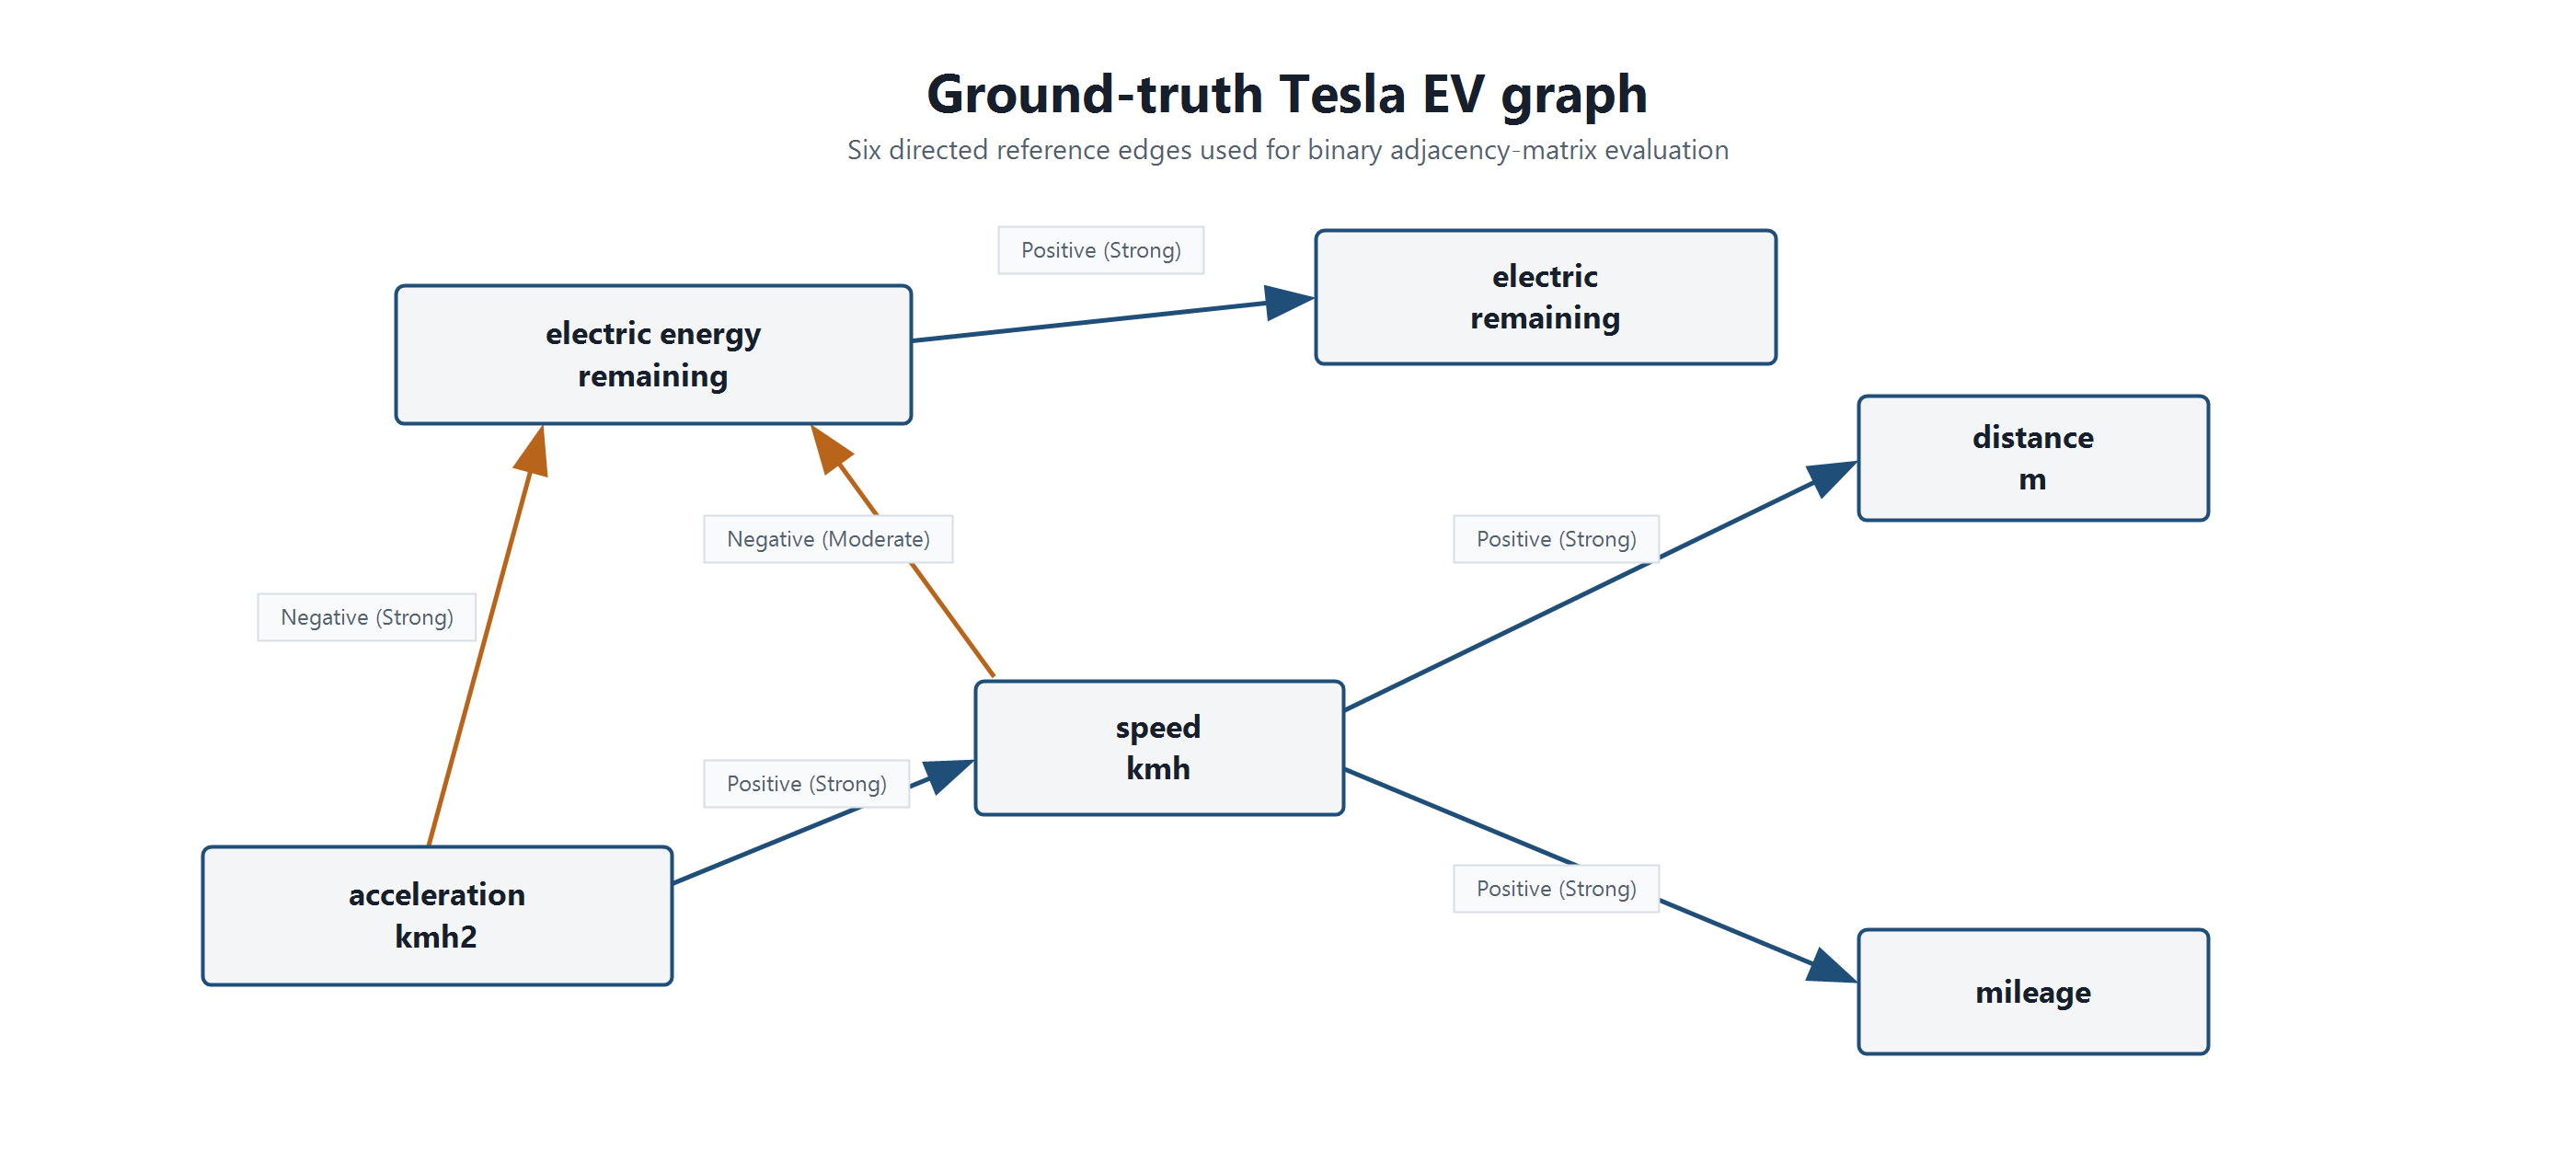
\includegraphics[width=0.86\textwidth]{figures/Ground_Truth_UC_Tesla_Energy_Consumption.png}%
  }{%
    \fbox{\parbox{0.82\textwidth}{Ground-truth DAG image not found. The edge list is shown in Table~\ref{tab:ground-truth-edges}.}}%
  }
  \caption{Ground-truth Tesla EV graph used as the evaluation target. The figure corresponds to the edge list in Table~\ref{tab:ground-truth-edges}.}
  \label{fig:ground-truth-dag}
\end{figure}

\section{Scope and Boundaries}

The graph-recovery task has three boundaries. First, it is single-dataset: all
primary results use the Tesla EV use case. Second, it is prompt-based: the
models are not fine-tuned and no external tool is called during generation.
Third, it is single-output per evaluated cell in the supplied artifacts: the
sidecar JSON files report \texttt{n\_runs = 1}. The notebook contains
repeated-run and self-consistency machinery, but the primary result directory
used in this thesis does not provide executed repeated-run evidence.

Earlier governance-oriented infrastructure remains relevant as supplementary
context. It motivated careful treatment of telemetry fields and local
inference, while the main chapters evaluate graph-recovery performance rather
than disclosure or utility trade-off metrics.

  \chapter{Methodology}
\label{sec:methodology}

\section{Overview of the Concept}
\label{sec:research-design}

The methodology evaluates LLM-assisted graph recovery as a controlled
comparison between model choice and prompt strategy. Every model-strategy cell
uses the same Tesla EV feature set, dataset fingerprint, ground-truth graph,
parser, and metric suite. The independent variables are the model and the
prompting strategy; the dependent variables are graph-recovery metrics
computed from the predicted and reference adjacency matrices.

Let \(V\) be the ordered set of six telemetry features. The ground-truth graph
is denoted \(G^\ast=(V,E^\ast)\), where \(E^\ast\) contains the six directed
reference edges. For a model \(m\) and strategy \(s\), the parsed LLM output is
denoted \(\hat{G}_{m,s}=(V,\hat{E}_{m,s})\). The corresponding binary
adjacency matrices are \(A^\ast\) and \(\hat{A}_{m,s}\), where an entry of 1
at row \(i\), column \(j\) indicates a directed edge from feature \(i\) to
feature \(j\). Evaluation consists of comparing \(\hat{A}_{m,s}\) with
\(A^\ast\).

The scientific object is therefore not a free-form answer quality judgment. It
is a directed edge set. Each LLM output is reduced to relationships of the
form \texttt{source -> target}, filtered to the six allowed feature names, and
converted into a binary adjacency matrix. This makes it possible to report
precision, recall, F1 score, structural Hamming distance, false discovery
rate, Pearson correlation, Hamming distance, and Frobenius norm for every
model-strategy combination.

\summarynote{Methodology map}{The methodology begins with a normalized Tesla
EV feature view, constructs a compact statistical fingerprint, prompts local
LLMs to output directed edges, parses the edges into adjacency matrices, and
evaluates those matrices against the ground-truth DAG.}

\section{Prompt-to-Graph Pipeline}

Figure~\ref{fig:graph-recovery-pipeline} summarizes the conceptual framework.
The implementation is materialized in the notebook and result directory as
\texttt{.json}, \texttt{.npy}, \texttt{.csv}, \texttt{.png}, and
\texttt{.jsonld} artifacts.

\begin{figure}[!htbp]
  \centering
  \begingroup
  \newcommand{\pipelinebox}[1]{%
    \fcolorbox{thesisline}{thesisgray}{%
      \parbox[c][13mm][c]{0.19\textwidth}{\centering\small\bfseries #1}%
    }%
  }
  \setlength{\tabcolsep}{2.5pt}
  \begin{tabular}{@{}ccccccc@{}}
    \pipelinebox{Telemetry\\data} &
    \(\rightarrow\) &
    \pipelinebox{Prompt strategy\\layer} &
    \(\rightarrow\) &
    \pipelinebox{LLM graph\\proposal} &
    \(\rightarrow\) &
    \pipelinebox{Edge\\parser} \\
    &&&&&& \(\downarrow\) \\
    \multicolumn{3}{c}{} &&
    \pipelinebox{Graph-recovery\\metrics} &
    \(\leftarrow\) &
    \pipelinebox{Ground-truth\\comparison} \\
    &&&&&& \(\uparrow\) \\
    \multicolumn{5}{c}{} &&
    \pipelinebox{Adjacency\\matrix}
  \end{tabular}
  \endgroup
  \caption{Conceptual prompt-to-graph framework used in the thesis. Telemetry features are transformed into a prompted graph proposal, parsed into an adjacency matrix, and compared with the ground-truth DAG to compute graph-recovery metrics.}
  \label{fig:graph-recovery-pipeline}
\end{figure}

\begin{table}[!htbp]
  \centering
  \small
  \setlength{\tabcolsep}{3pt}
  \begin{tabularx}{\textwidth}{@{}L{34mm}Y Y@{}}
    \toprule
    Stage & Operation & Repository trace \\
    \midrule
    Dataset loading & Load the normalized Tesla EV CSV and keep the configured six features. & Notebook dataset configuration; local copy at \path{data/tesla.csv}. \\
    Fingerprinting & Summarize per-feature count, mean, standard deviation, minimum, median, maximum, and Spearman rank correlations. & \texttt{dataset\_fingerprint} in the supervisor notebook. \\
    Prompt construction & Combine feature descriptions, dataset fingerprint, and one prompt strategy. & \texttt{make\_base\_prompt} and \texttt{STRATEGIES}. \\
    Inference & Call local Ollama models using bounded generation settings. & \texttt{call\_ollama}; per-cell result JSON files. \\
    Parsing & Extract directed edges from the raw LLM response and normalize feature tokens. & \texttt{parse\_causal\_edges}. \\
    Matrix conversion & Convert parsed edges into a binary adjacency matrix using the fixed feature order. & \texttt{edges\_to\_adjacency}; saved \texttt{.npy} files. \\
    Evaluation & Compare predicted and ground-truth matrices using eight graph metrics. & \path{evaluation_matrix_tesla_ev.csv} and \path{evaluation_matrix_tesla_ev_long.csv}. \\
    Export & Save graph plots, edge tables, consensus edges, and JSON-LD. & \path{edges_kg.csv}, \path{edges_kg.jsonld}, and \path{consensus_tesla_ev.csv}. \\
    \bottomrule
  \end{tabularx}
  \caption{Methodological pipeline and repository traceability. Each stage is tied to an artifact or function in the supervisor-provided notebook and result directory.}
  \label{tab:graph-pipeline}
\end{table}

\section{Dataset Fingerprint}

The LLM is not prompted with all 65,261 rows. Instead, the notebook constructs
a compact textual fingerprint of the selected features. The fingerprint
contains two parts:

\begin{itemize}
  \item per-feature descriptive statistics: count, mean, standard deviation,
  minimum, median, and maximum, rounded for compactness;
  \item a Spearman rank-correlation matrix over the six selected telemetry
  features.
\end{itemize}

This design gives the model structured information about the dataset without
placing the full table into the prompt. It also keeps the input consistent
across strategies. Any observed difference between strategies is therefore
attributable to instruction structure rather than different data exposure.

The fingerprint is not a causal discovery algorithm. It summarizes marginal
distributions and rank correlations. The LLM then uses that information,
feature names, and prompt instructions to propose directed edges; direction is
evaluated only after parsing against the ground-truth DAG.

\section{Output Parsing and Matrix Construction}

The parser is intentionally tolerant of common LLM formatting variation. It
accepts ASCII arrows and related arrow glyphs, removes simple markdown or JSON
fences, attempts to read JSON objects containing edge lists, normalizes feature
tokens by case and punctuation, and handles chained expressions such as
\texttt{A -> B -> C} as adjacent directed edges. It then discards any edge
whose source or target is not one of the six allowed features.

The parser output is \(\hat{E}_{m,s}\), the predicted set of directed feature
pairs for one model-strategy cell. Duplicate edges are removed, and self-loops
are not retained. The remaining edges are converted into \(\hat{A}_{m,s}\)
using the fixed Tesla EV feature order:

\begin{center}
\small
\begin{tabular}{@{}lll@{}}
\texttt{electricenergyremaining} & \texttt{electricremaining} & \texttt{speed\_kmh} \\
\texttt{acceleration\_kmh2} & \texttt{mileage} & \texttt{distance\_m}
\end{tabular}
\end{center}

This parser-centered design matters because the evaluation is performed on
matrices, not on prose. If the model gives a relationship in an unsupported
format or uses a feature name outside the allowed set, that content cannot
contribute to a correct edge. The thesis therefore evaluates both relational
knowledge and compliance with the machine-readable output contract.

\section{Result Artifacts Used as Source of Truth}

The main methodology and results use the repository-local artifact folder:

\begin{quote}
\path{results/tesla_ev_graph_recovery}
\end{quote}

The most important files are listed in Table~\ref{tab:method-artifacts}. These
files are used instead of rerunning the experiment, and no numerical claims
are introduced beyond what they support.

\begin{table}[!htbp]
  \centering
  \small
  \setlength{\tabcolsep}{3pt}
  \begin{tabularx}{\textwidth}{@{}L{58mm}Y@{}}
    \toprule
    Artifact & Methodological role \\
    \midrule
    \path{Ground_Truth_UC_Tesla_Energy_Consumption_signed.json} & Documents the six-feature ground-truth graph and signed edge labels. \\
    \path{Ground_Truth_UC_Tesla_Energy_Consumption_adjacency_matrix.npy} & Matrix target used for metric computation. \\
    \path{tesla_ev/<model>/<strategy>.json} & Stores raw model output, parsed edges, score dictionary, latency, and \texttt{n\_runs}. \\
    \path{tesla_ev/<model>/<strategy>.npy} & Stores the predicted adjacency matrix for a model-strategy cell. \\
    \path{evaluation_matrix_tesla_ev.csv} & Wide evaluation table with one row per model-strategy cell and eight metric columns. \\
    \path{evaluation_matrix_tesla_ev_long.csv} & Long-format version with explicit dataset, model, family, and strategy metadata. \\
    \path{edges_kg.csv} and \path{edges_kg.jsonld} & Predicted edge exports for knowledge-graph style inspection. \\
    \path{consensus_tesla_ev.csv} & Edge support table aggregating votes across evaluated model-strategy cells. \\
    \bottomrule
  \end{tabularx}
  \caption{Primary artifacts used as methodological and numerical source of truth. The thesis does not report unsupported results outside these files.}
  \label{tab:method-artifacts}
\end{table}

  \section{Prompt Strategy Design}
\label{sec:prompting}

Prompting is the experimental intervention. The dataset, feature set,
fingerprint, parser, ground truth, and metric suite remain fixed while the
instruction wrapper changes. The supervisor notebook originally contains a
larger strategy registry, but the validated primary results used in this
thesis contain five active strategies. Those five strategies are listed in
Table~\ref{tab:graph-prompting-strategies}.

\begin{table}[!htbp]
  \centering
  \scriptsize
  \setlength{\tabcolsep}{3pt}
  \begin{tabularx}{\textwidth}{@{}L{46mm}L{27mm}Y@{}}
    \toprule
    Strategy & Strategy role & Methodological purpose \\
    \midrule
    \shortstack[l]{\texttt{Strategy\_1}\\\texttt{Zero\_Shot\_Prompting}} & Zero-shot baseline & Uses the common base prompt without additional methodological framing. \\
    \shortstack[l]{\texttt{Strategy\_23}\\\texttt{No\_Instruction\_Control}} & Control baseline & Represents a neutral discovery instruction with no added causal-discovery policy beyond the base task. \\
    \shortstack[l]{\texttt{Strategy\_24}\\\texttt{Policy\_First\_Structured}} & Instruction structuring & Places explicit causal-discovery rules before the base task. \\
    \shortstack[l]{\texttt{Strategy\_25}\\\texttt{Least\_to\_Most}} & Prompt decomposition & Breaks graph recovery into ordered internal sub-problems from simpler physical links to more difficult accumulated-state links. \\
    \shortstack[l]{\texttt{Strategy\_26}\\\texttt{Skeleton\_of\_Thought}} & Prompt decomposition & Provides an internal answer skeleton covering energy-state edges, driving-behaviour edges, cross-group edges, and an integrity gate. \\
    \bottomrule
  \end{tabularx}
  \caption{Prompt strategies evaluated in the supervisor-provided Tesla EV results. The table uses the exact strategy names stored in the result CSV and JSON files.}
  \label{tab:graph-prompting-strategies}
\end{table}

\section{Common Base Prompt}

All evaluated strategies share a common graph-recovery scaffold. The base
prompt identifies the dataset as Tesla Full EV telematics, lists the six
features and their descriptions, supplies the dataset fingerprint, and asks
the model to identify directed feature relationships in the format
\texttt{feature\_a -> feature\_b}. The prompt explicitly requests one
relationship per line and no prose, numbering, or markdown. This output
contract is necessary because the downstream evaluator expects parseable
directed edges.

The base prompt is already a constrained analytics prompt. Therefore, the
comparison should not be interpreted as free-form language generation versus
structured generation. It is a comparison between different degrees and kinds
of instruction structure layered onto the same graph-recovery task.

\section{Baselines and Controls}

\subsection{Zero-Shot Prompting}

\strategy{Strategy_1_Zero_Shot_Prompting} applies the common base prompt
directly. It is called zero-shot because it provides no examples of correct
edges and no additional decomposition beyond the task instruction. It measures
how much graph-recovery performance the model can achieve from feature
semantics, dataset statistics, and the base output contract alone.

\subsection{No-Instruction Control}

\strategy{Strategy_23_No_Instruction_Control} is a neutral control condition.
In the active supervisor configuration, it also uses the base discovery prompt
without an added policy or decomposition layer. Its role is to provide an
additional control point for the adapted strategy set. Because it is close to
the zero-shot condition, differences between these two rows should be
interpreted conservatively and through the saved artifacts rather than treated
as evidence of a fundamentally different method.

\section{Instruction Structuring}

\strategy{Strategy_24_Policy_First_Structured} places a numbered
causal-discovery policy before the base task. The policy instructs the model
to report only direct relationships, reject correlation-only or co-movement
links, avoid bidirectional edges unless independently physically justified,
and keep the output to one ASCII-arrow edge per line.

The intended mechanism is constraint salience. By putting methodological rules
before the dataset description and task, the prompt attempts to make
directness, interventionability, and output format part of the task frame.
This is different from prompt decomposition: the policy-first prompt does not
split the task into stages, but it does make the evaluation criteria explicit
before generation.

\section{Prompt Decomposition}

Prompt decomposition strategies ask the model to organize the graph-recovery
problem into internal sub-tasks before producing the final edge list. In this
thesis, decomposition is evaluated through least-to-most prompting and
skeleton-of-thought prompting. The implementation requests only the final
edges, so the thesis evaluates observable output rather than hidden reasoning.

\subsection{Least-to-Most Prompting}

\strategy{Strategy_25_Least_to_Most} decomposes the graph-recovery problem
from simpler to more difficult sub-problems. The prompt asks the model to:
identify obvious physical edges, add edges supported by a physical law, add
edges involving accumulated state such as mileage or degradation, remove
correlation-only or mediated links, and output only the surviving final edges.

This strategy is relevant to telematics because vehicle-system relationships
are not all equally difficult. Some relationships, such as acceleration and
speed, are direct and physically familiar. Others, such as the relation
between driving behaviour and remaining energy, require integration across
energy and motion features. Least-to-most prompting tests whether an ordered
reasoning scaffold improves graph recovery compared with simpler baselines.

\subsection{Skeleton-of-Thought Prompting}

\strategy{Strategy_26_Skeleton_of_Thought} provides an internal answer
skeleton. The skeleton separates the candidate graph into energy-state edges,
driving-behaviour edges, cross-group edges, and an integrity gate that checks
for directness, correlation-only links, and invalid bidirectionality. The
model is then instructed to output only the merged final list of edges.

This strategy is more structured than least-to-most prompting because it
groups the feature graph by subsystem. In the Tesla EV task, this grouping is
natural: energy-related variables and driving-behaviour variables are
distinct, but the graph also contains cross-group relationships from speed and
acceleration to remaining energy. The strategy tests whether such an explicit
skeleton helps the model cover the graph without losing the output-format
constraint.

\section{Prompting Methods Outside the Primary Evidence}

The supervisor notebook contains commented or auxiliary strategy definitions,
including self-consistency and repeated-run machinery. Those definitions are
not treated as primary evaluated methods here because the JSON sidecars in the
validated result directory report \texttt{n\_runs = 1} for the model-strategy
cells used in the thesis. The thesis therefore does not claim measured
self-consistency improvements. It focuses on the five prompt strategies that
appear in \path{evaluation_matrix_tesla_ev_long.csv}.

  \section{Evaluation Metrics}
\label{sec:metrics}

The evaluation compares a predicted adjacency matrix \(\hat{A}_{m,s}\) with
the ground-truth adjacency matrix \(A^\ast\). Both matrices are binary and use
the same six-feature ordering. A value of 1 at row \(i\), column \(j\) means
that the source feature \(i\) has a directed relationship to the target
feature \(j\). The supervisor notebook binarizes matrices with a threshold of
0.5, which is equivalent to reading the saved 0/1 adjacency matrices
directly.

The metric suite contains eight values. Four metrics are edge-classification
metrics over the flattened adjacency matrix. Four metrics summarize structural
or matrix-level agreement. Table~\ref{tab:graph-metrics} gives the evaluation
role of each metric.

\begin{table}[!htbp]
  \centering
  \small
  \setlength{\tabcolsep}{3pt}
  \begin{tabularx}{\textwidth}{@{}L{36mm}L{26mm}Y@{}}
    \toprule
    Metric & Direction & Interpretation \\
    \midrule
    Precision & Higher is better & Fraction of predicted edges that are present in the ground truth. \\
    Recall & Higher is better & Fraction of ground-truth edges recovered by the model output. \\
    F1 Score & Higher is better & Harmonic mean of precision and recall; the headline edge-recovery balance. \\
    SHD & Lower is better & Structural Hamming distance; count of entries where predicted and ground-truth adjacency matrices differ. \\
    FDR & Lower is better & False discovery rate; fraction of predicted edges that are false positives. \\
    Pearson Correlation & Higher is better & Correlation between flattened predicted and ground-truth adjacency matrices, with undefined constant cases mapped to 0. \\
    Hamming Distance & Lower is better & Fraction of flattened adjacency entries that differ. \\
    Frobenius Norm & Lower is better & Matrix norm of the binary difference \(P-G\); numerically equal to \(\sqrt{\mathrm{SHD}}\) for binary matrices. \\
    \bottomrule
  \end{tabularx}
  \caption{Graph-recovery metrics used in the supervisor-provided evaluation matrix. The suite combines edge-level classification metrics with matrix-level structural agreement measures.}
  \label{tab:graph-metrics}
\end{table}

\subsection{Confusion Counts}

Let \(\hat{A}_{ij}\) be the predicted adjacency entry for one model-strategy
cell and \(A^\ast_{ij}\) the ground-truth entry. The flattened matrices define
four counts:

\begin{align}
  TP &= \sum_{i,j} \mathbb{1}[\hat{A}_{ij}=1 \wedge A^\ast_{ij}=1],\\
  FP &= \sum_{i,j} \mathbb{1}[\hat{A}_{ij}=1 \wedge A^\ast_{ij}=0],\\
  FN &= \sum_{i,j} \mathbb{1}[\hat{A}_{ij}=0 \wedge A^\ast_{ij}=1],\\
  TN &= \sum_{i,j} \mathbb{1}[\hat{A}_{ij}=0 \wedge A^\ast_{ij}=0].
\end{align}

These counts are computed over all matrix cells, including non-edge cells.
Because the graph is sparse, metrics must be interpreted carefully. Accuracy
is not reported as a headline metric because a model can obtain many true
negatives simply by predicting few or no edges. Precision, recall, F1, and
structural error are more informative for this task.

\subsection{Precision, Recall, and F1 Score}

Precision measures how many predicted edges are correct:

\begin{equation}
  \mathrm{Precision} = \frac{TP}{TP + FP}.
\end{equation}

Recall measures how many ground-truth edges are recovered:

\begin{equation}
  \mathrm{Recall} = \frac{TP}{TP + FN}.
\end{equation}

The F1 score balances precision and recall:

\begin{equation}
  \mathrm{F1} =
  \frac{2 \cdot \mathrm{Precision} \cdot \mathrm{Recall}}
       {\mathrm{Precision} + \mathrm{Recall}}.
\end{equation}

The notebook uses zero-division handling: if a denominator is zero, the
corresponding score is set to 0. This matters for cells where a model produces
no correct predicted edges or no predicted edges after parsing.

\subsection{Structural Hamming Distance}

Structural Hamming distance is the number of adjacency entries that differ:

\begin{equation}
  \mathrm{SHD} = \sum_{i,j} \mathbb{1}[\hat{A}_{ij} \neq A^\ast_{ij}].
\end{equation}

In this binary directed-graph setting, SHD counts both missed ground-truth
edges and extra predicted edges. It is useful because it reports absolute
structural error rather than only a precision-recall balance. A low SHD means
the predicted matrix is close to the target matrix; a high SHD means many
edge/non-edge decisions differ.

\subsection{False Discovery Rate}

False discovery rate is the fraction of predicted edges that are not in the
ground truth:

\begin{equation}
  \mathrm{FDR} = \frac{FP}{TP + FP}.
\end{equation}

When no edges are predicted, the supervisor notebook sets FDR to 0. This
convention avoids division by zero but requires careful interpretation:
zero FDR does not necessarily indicate a useful model if recall and F1 are
also zero.

\subsection{Pearson Correlation}

Pearson correlation is computed between the flattened binary predicted matrix
and the flattened binary ground-truth matrix. It captures linear agreement
between edge patterns. The notebook maps undefined cases to 0 when either
flattened vector is constant or the correlation is not a number. This
conservative fallback prevents degenerate outputs from producing undefined
metric values.

\subsection{Hamming Distance and Frobenius Norm}

Hamming distance is the fraction of flattened matrix entries that differ:

\begin{equation}
  \mathrm{Hamming}(\hat{A},A^\ast) =
  \frac{1}{n^2}\sum_{i,j}\mathbb{1}[\hat{A}_{ij} \neq A^\ast_{ij}].
\end{equation}

For the six-feature task, \(n=6\), so the denominator is 36. Hamming distance
is therefore a normalized version of structural error.

The Frobenius norm is:

\begin{equation}
  \lVert \hat{A}-A^\ast\rVert_F =
  \sqrt{\sum_{i,j}(\hat{A}_{ij}-A^\ast_{ij})^2}.
\end{equation}

Because the matrices are binary, this value is the square root of the number
of differing entries. It provides a matrix-error magnitude that is consistent
with SHD while using a standard matrix norm.

\section{Metric Interpretation}

No single metric is sufficient. Precision can be high when a model predicts
few edges, recall can be high when a model predicts many edges, and F1 can
hide whether the errors are mainly false positives or false negatives. SHD,
Hamming distance, and Frobenius norm expose total matrix error. FDR exposes
how much of the predicted graph is spurious. Pearson correlation provides an
additional matrix-level agreement signal.

The results chapter therefore reports rankings and interpretation across the
metric suite rather than treating one number as a universal quality score. F1
is useful as the primary edge-recovery balance, but the thesis also examines
false discovery and structural error because fleet-monitoring graphs can be
misleading when they contain plausible but unsupported directed links.

  \section{Experimental Setup}
\label{sec:experimental-setup}

The primary experiment is the supervisor-provided Tesla EV graph-recovery run
stored under \path{results/tesla_ev_graph_recovery}. The thesis analyzes the
saved experimental evidence rather than introducing a new benchmark run.

\subsection{Models}

The evaluated models are local Ollama models:
\texttt{deepseek-r1:8b} and \texttt{llama3.1:8b}. The supervisor notebook
records both as 4.9 GB models and labels their families as DeepSeek and Llama,
respectively. Table~\ref{tab:graph-models} summarizes the model configuration
used in the primary result matrix.

\begin{table}[!htbp]
  \centering
  \small
  \setlength{\tabcolsep}{3pt}
  \begin{tabularx}{\textwidth}{@{}L{32mm}L{24mm}L{22mm}Y@{}}
    \toprule
    Model & Family & Size in result CSV & Role in comparison \\
    \midrule
    \texttt{deepseek-r1:8b} & DeepSeek & 4.9 GB & Reasoning-oriented open-source model evaluated for structured graph recovery. \\
    \texttt{llama3.1:8b} & Llama & 4.9 GB & Same-size open-source baseline model for comparison. \\
    \bottomrule
  \end{tabularx}
  \caption{Models evaluated in the supervisor-provided Tesla EV result matrix. The size and family fields are taken from the long-format evaluation CSV.}
  \label{tab:graph-models}
\end{table}

The notebook calls Ollama through \path{/api/generate}. It sets temperature to
0.2, top-\(p\) to 0.9, and context length to 8192 in the notebook
configuration. It also defines a per-model output-token cap for
\texttt{deepseek-r1:8b} to prevent reasoning traces from running without a
known bound. These settings are documented as part of the supervisor notebook;
the result artifacts, rather than a new run, are the numerical source of
truth.

\subsection{Dataset and Run Grid}

The active dataset list contains one dataset:
\texttt{tesla\_ev}, labeled \emph{Tesla Full EV}. The active model list
contains two models. The validated result matrix contains five strategies.
Therefore, the primary evaluation matrix has ten rows:

\begin{equation}
  1 \text{ dataset} \times 2 \text{ models} \times 5 \text{ strategies}
  = 10 \text{ model-strategy cells}.
\end{equation}

Each cell is represented by one predicted adjacency matrix in the result
directory. The JSON sidecars report \texttt{n\_runs = 1}. The folder name
contains \texttt{10x}, and the notebook includes repeated-run code, but the
validated primary files used for this thesis do not provide repeated-run
metric rows. The methodology therefore treats the experiment as a
single-output-per-cell comparison.

\begin{table}[!htbp]
  \centering
  \small
  \setlength{\tabcolsep}{3pt}
  \begin{tabularx}{\textwidth}{@{}L{45mm}Y@{}}
    \toprule
    Configuration item & Value used in primary thesis evidence \\
    \midrule
    Dataset key & \texttt{tesla\_ev} \\
    Dataset label & Tesla Full EV \\
    Use-case name & \texttt{UC\_Tesla\_Energy\_Consumption} \\
    Selected features & Six: \texttt{electricenergyremaining}, \texttt{electricremaining}, \texttt{speed\_kmh}, \texttt{acceleration\_kmh2}, \texttt{mileage}, \texttt{distance\_m} \\
    Models & \texttt{deepseek-r1:8b}, \texttt{llama3.1:8b} \\
    Strategies in primary results & Five \\
    Evaluation rows & Ten model-strategy cells \\
    Per-cell repetitions in JSON sidecars & \texttt{n\_runs = 1} \\
    Primary result table & \path{evaluation_matrix_tesla_ev_long.csv} \\
    \bottomrule
  \end{tabularx}
  \caption{Primary experimental configuration used in the thesis. The table intentionally avoids unsupported repeated-run claims.}
  \label{tab:primary-experiment-config}
\end{table}

\subsection{Saved Per-Cell Artifacts}

For each evaluated model-strategy cell, the result directory contains three
main artifacts:

\begin{itemize}
  \item a \texttt{.json} sidecar with the dataset key, model, strategy, feature
  list, parsed edges, metric scores, total latency, \texttt{n\_runs}, errors,
  and raw model text;
  \item a \texttt{.npy} file storing the predicted adjacency matrix used by the
  evaluation builder;
  \item a \texttt{.png} graph visualization of the predicted edge set.
\end{itemize}

The result directory also contains aggregate artifacts: the full evaluation
matrix, a long-format evaluation table, per-model and F1 heatmaps, a long edge
export, a JSON-LD edge export, and a consensus edge table. These artifacts
allow the results chapter to move between numerical ranking, qualitative edge
inspection, and consensus analysis without recomputing generations.

\subsection{Reproducibility Boundary}

The reproducibility standard is artifact traceability rather than experiment
rerun. Every numerical claim in the methodology and results must be traceable
to one of the following:

\begin{itemize}
  \item \path{evaluation_matrix_tesla_ev.csv};
  \item \path{evaluation_matrix_tesla_ev_long.csv};
  \item per-cell result JSON files under \path{tesla_ev/<model>/<strategy>.json};
  \item \path{Ground_Truth_UC_Tesla_Energy_Consumption_signed.json};
  \item \path{edges_kg.csv};
  \item \path{consensus_tesla_ev.csv}.
\end{itemize}

This boundary prevents the thesis from importing claims from commented
notebook cells, unexecuted repeated-run sections, or the older summarization
and governance-oriented experiment. The graph-recovery artifacts are primary;
previous repository infrastructure is supplementary.

\subsection{Known Methodological Limitations}

The experimental setup has several limitations that affect interpretation.
First, the evaluation uses one Tesla EV dataset and one six-feature graph, so
the result is not a general benchmark for all vehicle systems. Second, the
ground-truth graph is physics-informed and suitable for evaluation, but it is
not a formally identified causal model from interventions. Third, the
validated artifacts provide one output per model-strategy cell, so output
variance and self-consistency cannot be quantified from the primary evidence.
Fourth, the parser enforces a strict feature vocabulary; useful but
out-of-vocabulary prose does not become a correct edge.

These limitations do not invalidate the comparison. They define its scope:
the thesis evaluates prompt decomposition and instruction structure as
practical methods for improving LLM-assisted telematics graph recovery in a
controlled, auditable Tesla EV setting.

  \chapter{Results}
\label{sec:results}

\newcommand{\sZero}{\shortstack[l]{\texttt{S1}\\\mbox{Zero-shot}}}
\newcommand{\sControl}{\shortstack[l]{\texttt{S23}\\\mbox{No-instruction}}}
\newcommand{\sPolicy}{\shortstack[l]{\texttt{S24}\\\mbox{Policy-first}}}
\newcommand{\sLeast}{\shortstack[l]{\texttt{S25}\\\mbox{Least-to-most}}}
\newcommand{\sSkeleton}{\shortstack[l]{\texttt{S26}\\\mbox{Skeleton}}}

This chapter reports the Tesla EV graph-recovery results stored in
\path{results/tesla_ev_graph_recovery}. The primary numerical source is
\path{results/tesla_ev_graph_recovery/evaluation_matrix_tesla_ev_long.csv};
edge-level interpretation uses the per-cell JSON files,
\path{results/tesla_ev_graph_recovery/edges_kg.csv}, and
\path{results/tesla_ev_graph_recovery/consensus_tesla_ev.csv}. No additional
experiments are introduced.

\summarynote{Reading guide}{Higher precision, recall, F1, and Pearson
correlation are better. Lower SHD, FDR, Hamming distance, and Frobenius norm
are better. Because every validated JSON sidecar reports \texttt{n\_runs = 1},
the tables describe observed model-strategy outputs, not repeated-run
stability.}

\section{Evaluation Matrix Overview}

The primary result matrix contains ten rows: two models evaluated under five
prompt strategies on the Tesla Full EV use case. Table~\ref{tab:graph-results}
lists the complete metric set and should be read as a descriptive comparison,
because each row represents one validated model-strategy output. The strongest
observed row is
\texttt{deepseek-r1:8b} with
\strategy{Strategy_26_Skeleton_of_Thought}, which reaches precision 0.4444,
recall 0.6667, F1 score 0.5333, SHD 7, FDR 0.5556, Pearson correlation
0.4303, Hamming distance 0.1944, and Frobenius norm 2.6458.

\begin{table}[!htbp]
  \centering
  \scriptsize
  \setlength{\tabcolsep}{2.5pt}
  \renewcommand{\arraystretch}{1.10}
  \begin{tabularx}{\textwidth}{@{}L{25mm}L{34mm}rrrrrrrr@{}}
    \toprule
    Model & Strategy & Prec. & Rec. & F1 & SHD & FDR & Pearson & Hamm. & Frob. \\
    \midrule
    \texttt{deepseek-r1:8b} & \sZero & 0.0000 & 0.0000 & 0.0000 & 6 & 0.0000 & 0.0000 & 0.1667 & 2.4495 \\
    \texttt{deepseek-r1:8b} & \sControl & 0.3333 & 0.5000 & 0.4000 & 9 & 0.6667 & 0.2582 & 0.2500 & 3.0000 \\
    \texttt{deepseek-r1:8b} & \sPolicy & 0.0000 & 0.0000 & 0.0000 & 6 & 0.0000 & 0.0000 & 0.1667 & 2.4495 \\
    \texttt{deepseek-r1:8b} & \sLeast & 0.0000 & 0.0000 & 0.0000 & 6 & 0.0000 & 0.0000 & 0.1667 & 2.4495 \\
    \texttt{deepseek-r1:8b} & \sSkeleton & \textbf{0.4444} & \textbf{0.6667} & \textbf{0.5333} & 7 & 0.5556 & \textbf{0.4303} & 0.1944 & 2.6458 \\
    \addlinespace
    \texttt{llama3.1:8b} & \sZero & 0.3333 & 0.5000 & 0.4000 & 9 & 0.6667 & 0.2582 & 0.2500 & 3.0000 \\
    \texttt{llama3.1:8b} & \sControl & 0.2857 & 0.3333 & 0.3077 & 9 & 0.7143 & 0.1569 & 0.2500 & 3.0000 \\
    \texttt{llama3.1:8b} & \sPolicy & 0.1667 & 0.1667 & 0.1667 & 10 & 0.8333 & 0.0000 & 0.2778 & 3.1623 \\
    \texttt{llama3.1:8b} & \sLeast & 0.2222 & 0.3333 & 0.2667 & 11 & 0.7778 & 0.0861 & 0.3056 & 3.3166 \\
    \texttt{llama3.1:8b} & \sSkeleton & 0.2222 & 0.3333 & 0.2667 & 11 & 0.7778 & 0.0861 & 0.3056 & 3.3166 \\
    \bottomrule
  \end{tabularx}
  \caption{Complete Tesla EV graph-recovery evaluation matrix from the long-format evaluation CSV. Strategy labels are abbreviated for readability; values are copied without numerical modification.}
  \label{tab:graph-results}
\end{table}

\begin{figure}[p]
  \centering
  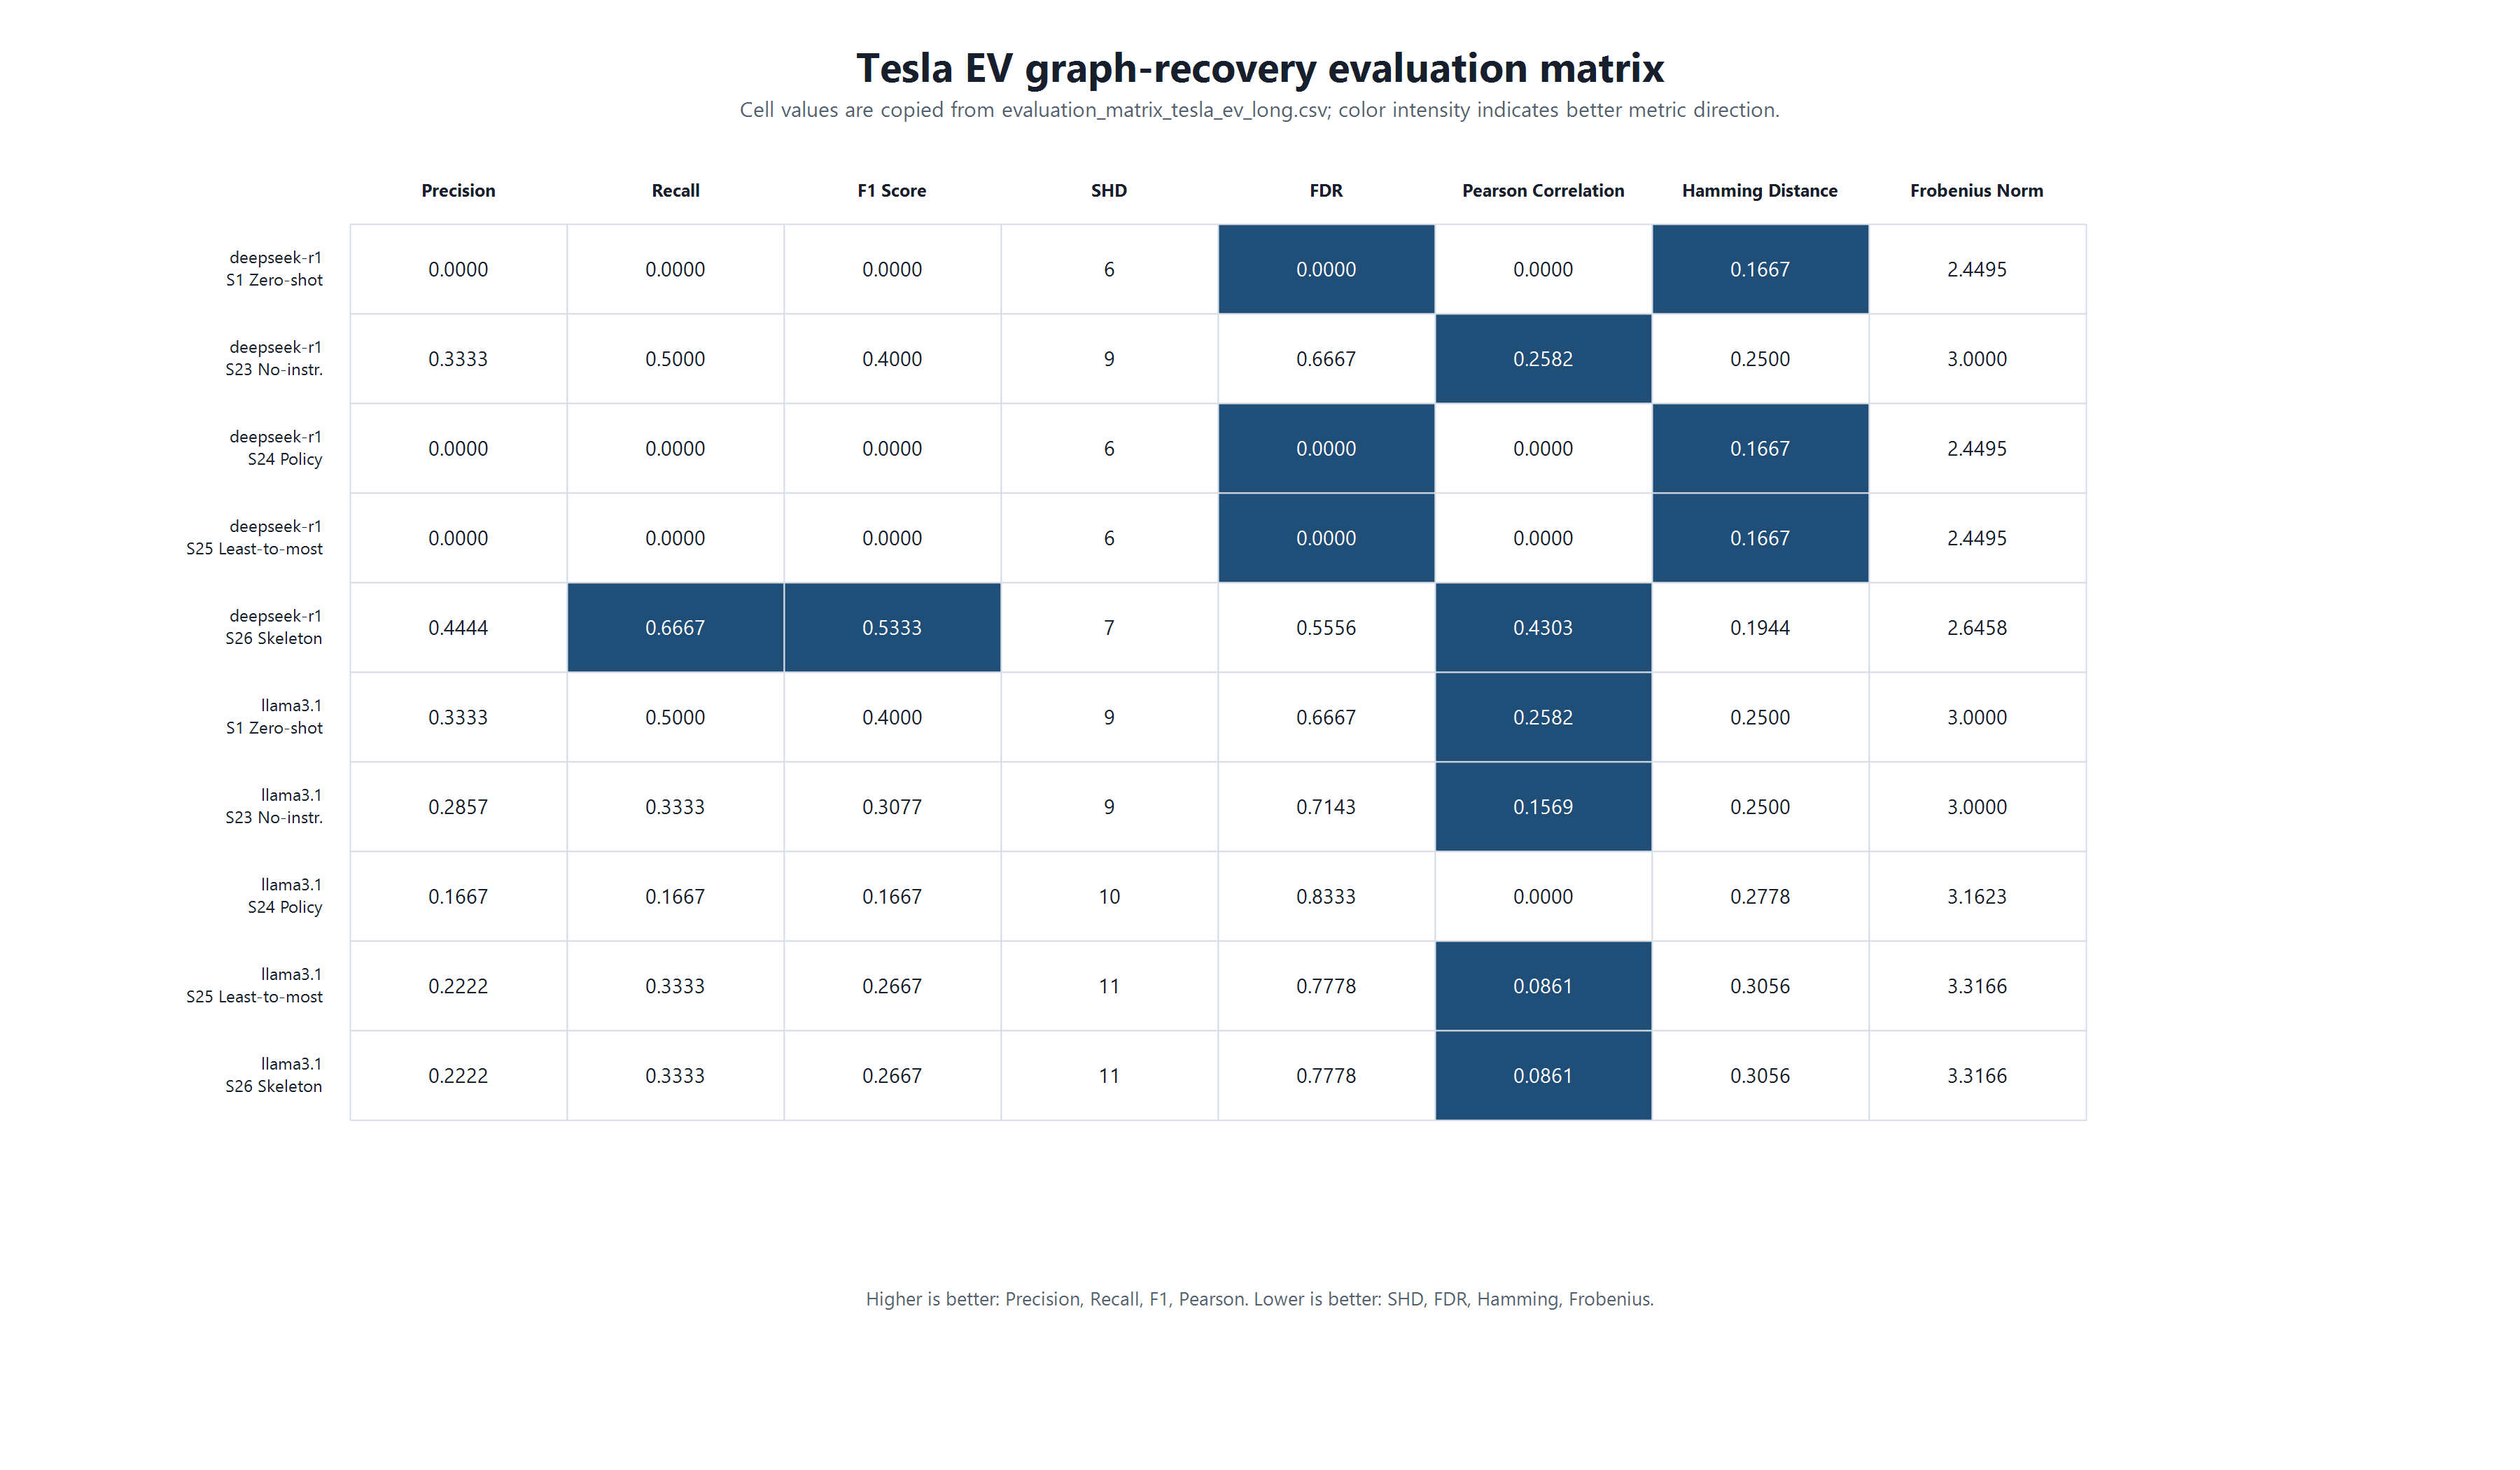
\includegraphics[width=\textwidth,height=0.62\textheight,keepaspectratio]{figures/evaluation_matrix_tesla_ev_heatmap.png}
  \caption{Evaluation matrix heatmap for the Tesla EV graph-recovery task. The visual summary complements Table~\ref{tab:graph-results} by showing how edge-recovery and structural-error metrics vary across model-strategy cells.}
  \label{fig:evaluation-matrix-heatmap}
\end{figure}

Figure~\ref{fig:evaluation-matrix-heatmap} makes the central pattern visible:
ranking is not monotonic with prompt complexity. The best row is a
decomposition-style strategy, yet several structured rows perform poorly.
DeepSeek with policy-first prompting and least-to-most prompting produces no
parseable predicted edges in the validated sidecars, yielding F1 score 0.0000.
Llama produces non-empty graphs in every evaluated strategy, but it often
overpredicts false edges.

\section{Model Comparison}

The two models show different failure profiles. Table~\ref{tab:model-average-results}
summarizes this contrast: averaged over the five prompt strategies, Llama has
higher mean F1 than DeepSeek, while DeepSeek has lower mean structural error.
This apparent tension is explained by empty outputs: three DeepSeek cells
predict no edges, which keeps SHD at 6 for those rows but also gives zero
recall and zero F1. Llama usually predicts edges, recovering more true
positives but also adding more false positives.

\begin{table}[!htbp]
  \centering
  \scriptsize
  \setlength{\tabcolsep}{3pt}
  \begin{tabular}{@{}lrrrrrr@{}}
    \toprule
    Model & Mean precision & Mean recall & Mean F1 & Mean SHD & Mean FDR & Mean Pearson \\
    \midrule
    \texttt{deepseek-r1:8b} & 0.1555 & 0.2333 & 0.1867 & 6.8000 & 0.2445 & 0.1377 \\
    \texttt{llama3.1:8b} & 0.2460 & 0.3333 & 0.2816 & 10.0000 & 0.7540 & 0.1175 \\
    \bottomrule
  \end{tabular}
  \caption{Model-level averages across the five evaluated strategies. The averages are descriptive because the experiment contains one output per model-strategy cell.}
  \label{tab:model-average-results}
\end{table}

DeepSeek is therefore not simply better or worse than Llama. It produces the
best single result under skeleton-of-thought prompting, but it also has three
zero-edge cells. Llama is more consistently non-empty but more prone to
spurious relationships, especially mileage-distance reversals and
energy-to-usage edges that are not in the ground truth.

\section{Strategy Comparison}

Table~\ref{tab:strategy-average-results} averages each strategy across both
models. Skeleton-of-thought has the highest mean F1 score, 0.4000, driven by
the strong DeepSeek skeleton result and the moderate Llama skeleton result.
The no-instruction control is second, with mean F1 0.3539. Policy-first
structured prompting is weakest by mean F1, 0.0834.

\begin{table}[!htbp]
  \centering
  \scriptsize
  \setlength{\tabcolsep}{3pt}
  \begin{tabular}{@{}lrrrrrr@{}}
    \toprule
    Strategy & Mean precision & Mean recall & Mean F1 & Mean SHD & Mean FDR & Mean Pearson \\
    \midrule
    \sSkeleton & 0.3333 & 0.5000 & 0.4000 & 9.0000 & 0.6667 & 0.2582 \\
    \sControl & 0.3095 & 0.4167 & 0.3539 & 9.0000 & 0.6905 & 0.2076 \\
    \sZero & 0.1667 & 0.2500 & 0.2000 & 7.5000 & 0.3334 & 0.1291 \\
    \sLeast & 0.1111 & 0.1667 & 0.1334 & 8.5000 & 0.3889 & 0.0431 \\
    \sPolicy & 0.0834 & 0.0834 & 0.0834 & 8.0000 & 0.4167 & 0.0000 \\
    \bottomrule
  \end{tabular}
  \caption{Strategy-level averages across DeepSeek and Llama3.1. Strategy labels use the same abbreviations as Table~\ref{tab:graph-results}; the ranking is descriptive and should not be read as a repeated-run result.}
  \label{tab:strategy-average-results}
\end{table}

\begin{figure}[p]
  \centering
  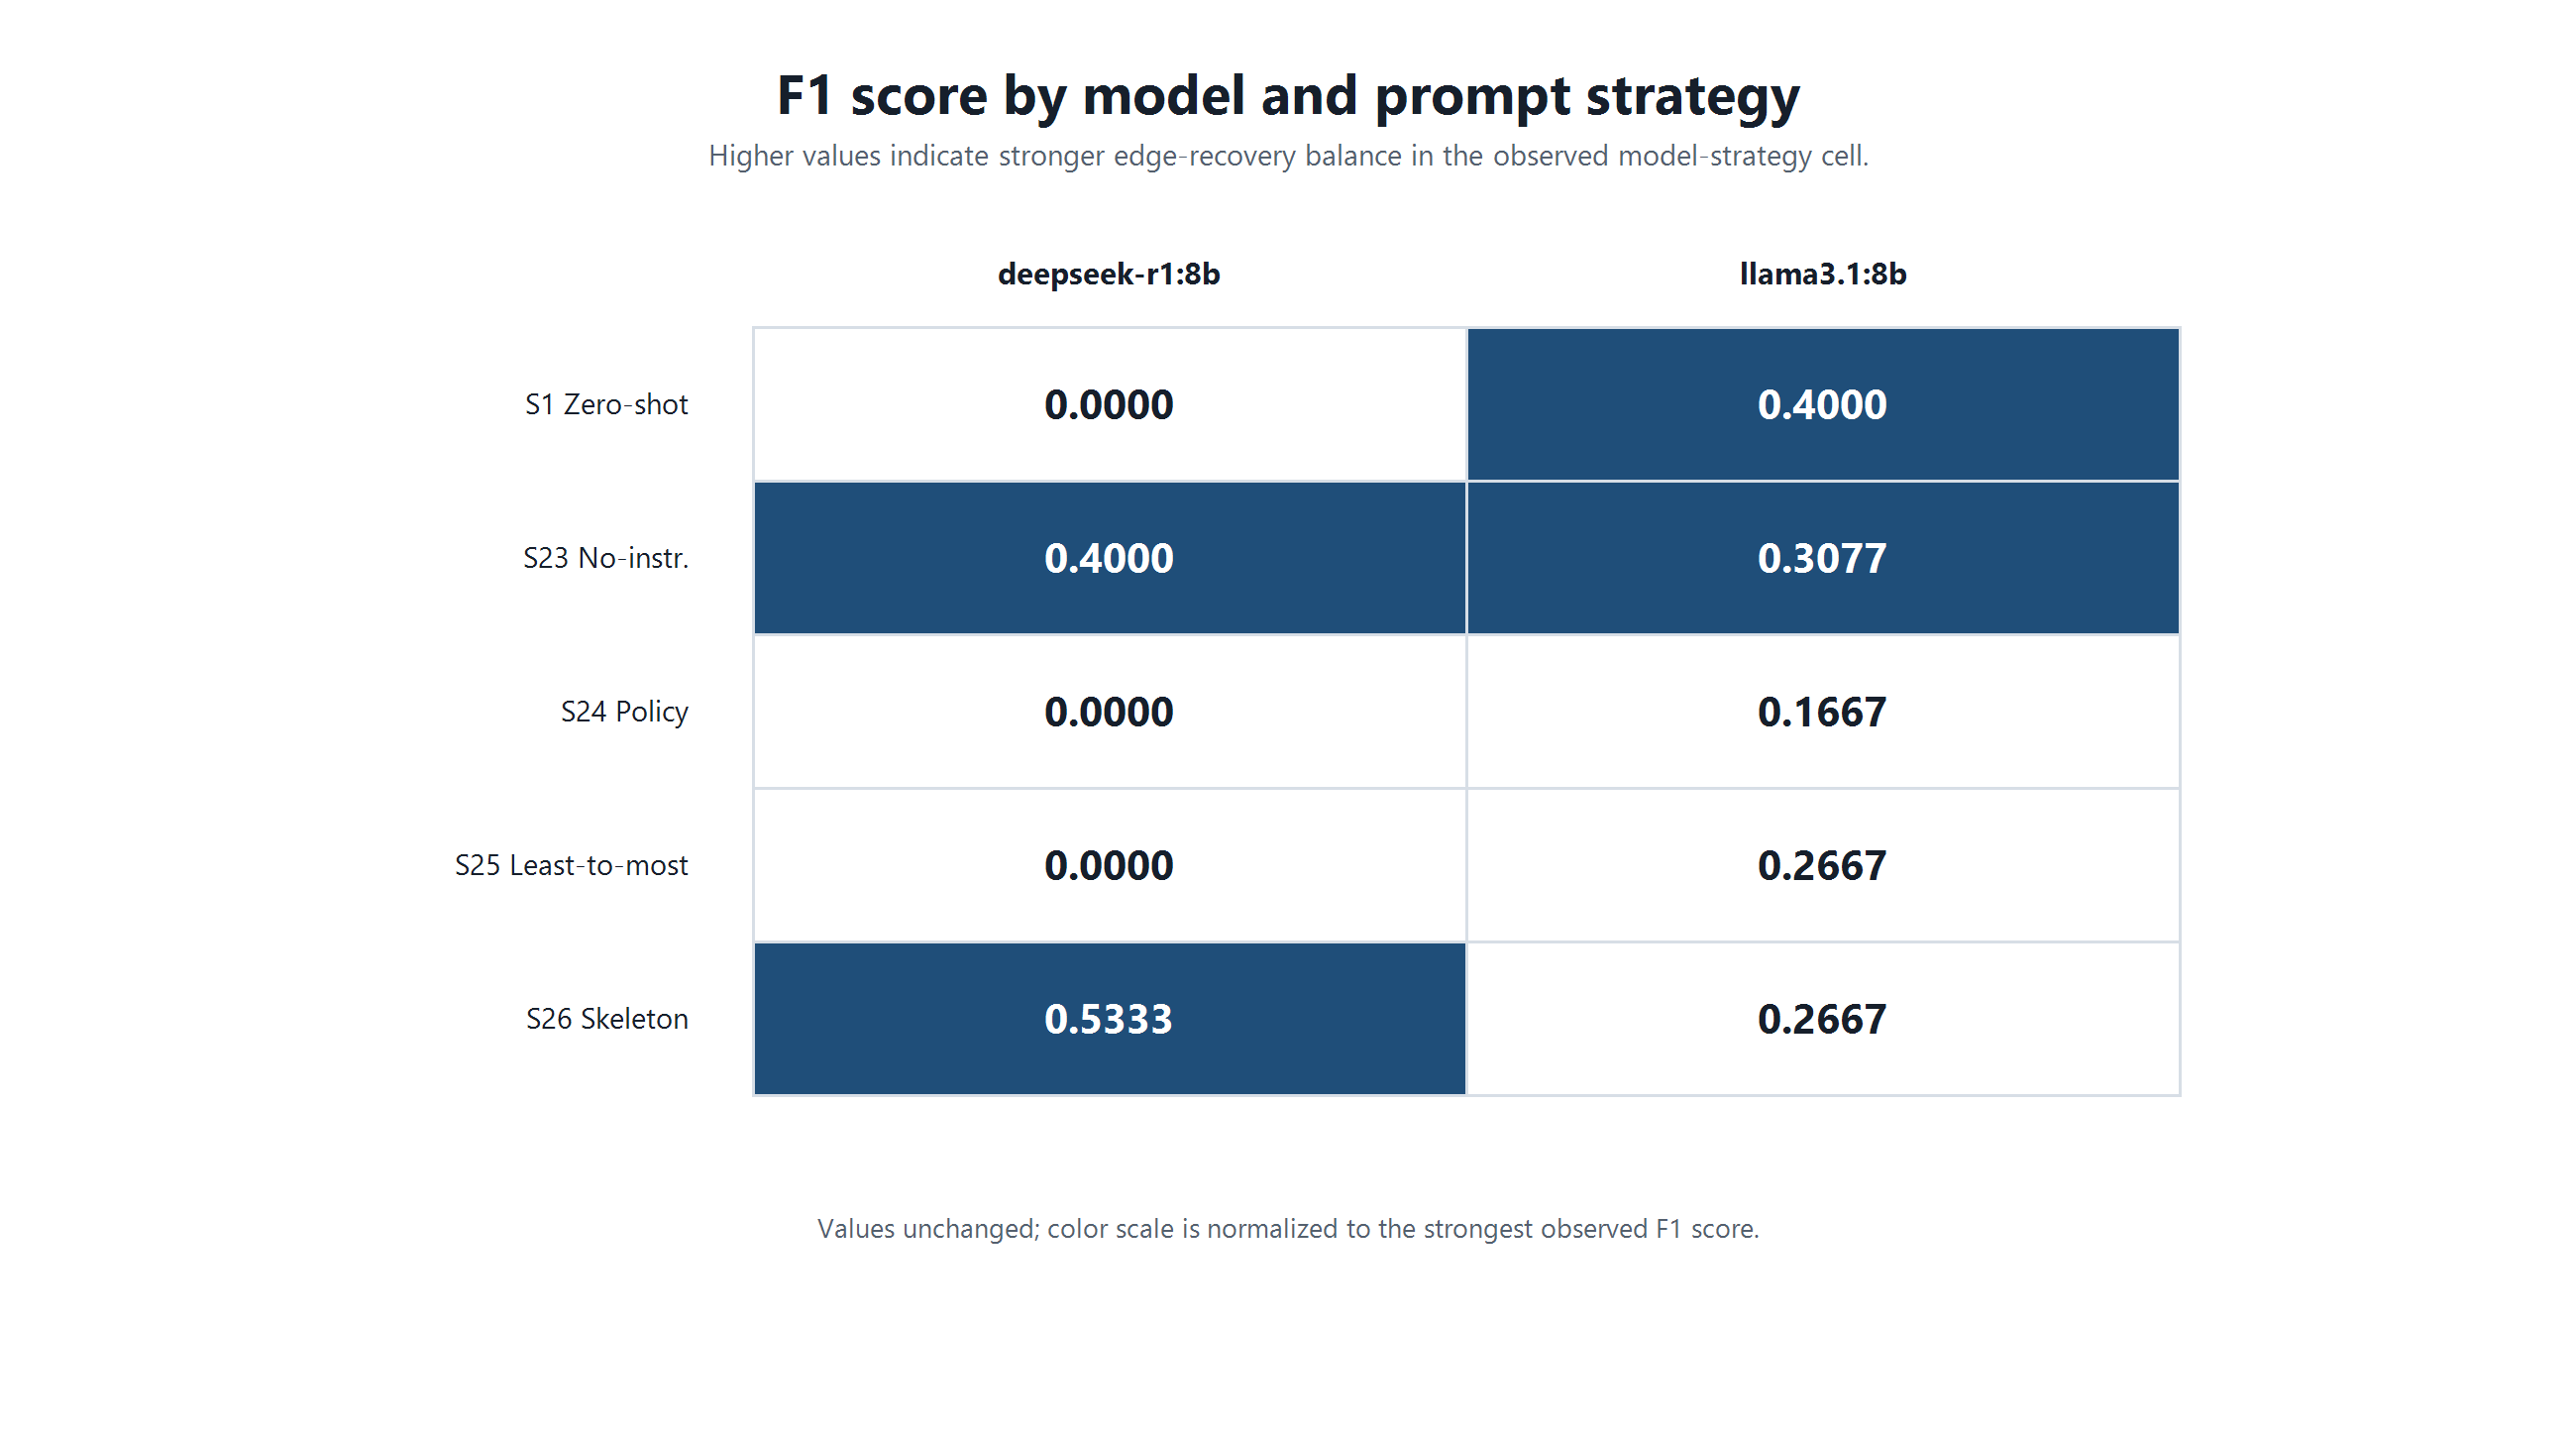
\includegraphics[width=\textwidth,height=0.58\textheight,keepaspectratio]{figures/f1_strategy_vs_model_tesla_ev.png}
  \caption{F1 heatmap by strategy and model. The strongest cell is DeepSeek with skeleton-of-thought prompting; the same figure also shows that the strategy effect differs by model.}
  \label{fig:f1-strategy-model}
\end{figure}

The decomposition evidence is therefore mixed but meaningful. As
Figure~\ref{fig:f1-strategy-model} shows, skeleton-of-thought is the best
strategy on average and gives the best overall cell. Least-to-most does not
show the same benefit: it produces an empty DeepSeek
output and a high-false-positive Llama output. The difference suggests that
decomposition is useful only when the decomposition structure matches the
model's output behavior and preserves the final edge-list contract.

\section{Edge-Level Analysis}

The best cell, DeepSeek with skeleton-of-thought, predicts nine edges. Four
are true positives and five are false positives. It recovers the
energy-to-range edge, the speed-to-distance edge, and the two driving-to-energy
edges. It misses \texttt{acceleration\_kmh2 -> speed\_kmh} and
\texttt{speed\_kmh -> mileage}. It also predicts false edges, including
\texttt{speed\_kmh -> acceleration\_kmh2},
\texttt{acceleration\_kmh2 -> distance\_m}, and
\texttt{distance\_m -> mileage}.

Table~\ref{tab:edge-level-results} summarizes the main edge-level patterns in
the representative cells used for interpretation.

\begin{table}[!htbp]
  \centering
  \scriptsize
  \setlength{\tabcolsep}{3pt}
  \renewcommand{\arraystretch}{1.12}
  \begin{tabularx}{\textwidth}{@{}L{31mm}rrrrY@{}}
    \toprule
    Model / strategy & Pred. & TP & FP & FN & Main edge-level pattern \\
    \midrule
    \shortstack[l]{\texttt{deepseek-r1:8b}\\\sSkeleton} & 9 & 4 & 5 & 2 & Best recovery; captures energy links and speed-to-distance, but reverses acceleration/speed and adds downstream energy/range edges. \\
    \shortstack[l]{\texttt{llama3.1:8b}\\\sZero} & 9 & 3 & 6 & 3 & Recovers three true edges but adds several reversed or energy-to-speed links. \\
    \shortstack[l]{\texttt{deepseek-r1:8b}\\\sControl} & 9 & 3 & 6 & 3 & Recovers three true edges but adds false links from \texttt{electricremaining} and a speed-to-acceleration reversal. \\
    \shortstack[l]{\texttt{llama3.1:8b}\\\sPolicy} & 6 & 1 & 5 & 5 & Retains only the energy-to-range ground-truth edge. \\
    \shortstack[l]{\texttt{deepseek-r1:8b}\\S1/S24/S25} & 0 & 0 & 0 & 6 & Empty raw outputs in the validated sidecars; no graph recovered. \\
    \bottomrule
  \end{tabularx}
  \caption{Edge-level interpretation of representative model-strategy cells. Counts are derived from per-cell JSON edge lists and the six-edge ground truth.}
  \label{tab:edge-level-results}
\end{table}

The most frequent false-positive pattern is direction reversal. The false edge
\texttt{speed\_kmh -> acceleration\_kmh2} appears in seven predicted edge
sets, while the ground truth contains the opposite direction
\texttt{acceleration\_kmh2 -> speed\_kmh}. Mileage and distance are also often
reversed: \texttt{mileage -> distance\_m} appears six times, and
\texttt{distance\_m -> mileage} appears five times, while the ground truth
contains \texttt{speed\_kmh -> mileage} and \texttt{speed\_kmh -> distance\_m}.

These errors are scientifically important. They show that the models often
identify semantically related feature pairs but fail to recover the evaluated
direction or the directness constraint. For fleet monitoring, that distinction
matters: a graph with plausible but reversed edges can mislead downstream
reasoning even if it appears domain-relevant.

\section{Consensus Graph}

The consensus file keeps edges that receive support from at least half of the
ten model-strategy cells. Five edges meet this threshold, shown in
Table~\ref{tab:consensus-results}. Only two of them are ground-truth edges.

\begin{table}[!htbp]
  \centering
  \small
  \setlength{\tabcolsep}{2pt}
  \begin{tabularx}{\textwidth}{@{}L{48mm}L{48mm}rrL{18mm}@{}}
    \toprule
    Source & Target & Votes & Support & Ground truth? \\
    \midrule
    \texttt{electricenergyremaining} & \texttt{electricremaining} & 7 & 0.7 & Yes \\
    \texttt{speed\_kmh} & \texttt{acceleration\_kmh2} & 7 & 0.7 & No \\
    \texttt{mileage} & \texttt{distance\_m} & 6 & 0.6 & No \\
    \texttt{acceleration\_kmh2} & \texttt{speed\_kmh} & 5 & 0.5 & Yes \\
    \texttt{distance\_m} & \texttt{mileage} & 5 & 0.5 & No \\
    \bottomrule
  \end{tabularx}
  \caption{Consensus edges from the supervisor-provided consensus CSV. Consensus identifies recurring model beliefs, but it does not guarantee correctness.}
  \label{tab:consensus-results}
\end{table}

The consensus graph therefore acts as an error-analysis tool rather than a
replacement for the ground truth. It highlights the robust
\texttt{electricenergyremaining -> electricremaining} relationship and the
\texttt{acceleration\_kmh2 -> speed\_kmh} relationship. It also amplifies
recurring mistakes: speed-to-acceleration and mileage-distance reversals are
popular enough to pass the consensus threshold.

\section{Summary of Findings}

The validated results support five findings:

\begin{itemize}
  \item skeleton-of-thought prompting with DeepSeek is the best single
  model-strategy cell by F1 score and Pearson correlation;
  \item Llama has higher average F1 across strategies, but also much higher
  average false discovery rate and structural error;
  \item DeepSeek is more brittle in this artifact set because three strategy
  cells contain empty raw outputs and zero predicted edges;
  \item prompt decomposition is not uniformly beneficial: skeleton-of-thought
  helps, while least-to-most does not improve the evaluated graph recovery;
  \item consensus edges reveal both stable true relationships and stable false
  beliefs, especially direction reversals.
\end{itemize}

These findings remain tied to the artifact set: one dataset, two models,
five active prompt strategies, and one validated output per model-strategy
cell.

  \chapter{Discussion}
\label{sec:discussion}

The results support a cautious but useful interpretation of prompt
decomposition for telematics graph recovery. The best observed configuration
is a decomposition-style prompt: \texttt{deepseek-r1:8b} with
\strategy{Strategy_26_Skeleton_of_Thought}. The broader evidence is not a
simple story that more structure always helps. Some structured strategies
produce empty outputs or many false positives, and the consensus graph
preserves recurring mistakes as well as recurring correct edges.

\section{Answering the Research Questions}

\subsection{RQ1: Model Ability to Recover Directed Relationships}

Both models recover some directed telemetry relationships, but neither
recovers the six-edge ground truth reliably. The strongest cell recovers four
of six ground-truth edges and predicts five additional false edges. Llama's
best cell recovers three of six ground-truth edges and also predicts six false
edges. These values show that local open-source LLMs can propose useful graph
fragments, especially for semantically salient energy and motion relations,
but they do not produce a sufficiently reliable graph without evaluation.

The most consistently recovered true edge is the energy-to-range relationship
from \texttt{electricenergyremaining} to \texttt{electricremaining}, which
appears in seven of the ten predicted edge sets. This is unsurprising because
the feature names strongly suggest a direct relation. Edges that require more
careful direction or directness judgment are less stable.

\subsection{RQ2: Prompt Decomposition Strategies}

Prompt decomposition has mixed results. Skeleton-of-thought is the strongest
strategy by mean F1 score across the two models and produces the best single
cell. Its subsystem-oriented skeleton appears to help DeepSeek connect
energy-state, driving-behaviour, and cross-group relationships. This is the
clearest positive evidence for decomposition in the thesis.

Least-to-most prompting does not show the same benefit. DeepSeek's
least-to-most sidecar contains an empty raw response and no parsed edges,
while Llama's least-to-most output contains many false positives. This
suggests that decomposition can fail in two different ways: it can make the
model fail to produce a parseable answer, or it can encourage a broad list of
plausible but unsupported links. Decomposition is therefore not a guarantee of
better graph recovery; it is a design variable that must be validated per
model and task.

\subsection{RQ3: Instruction Structuring}

Policy-first structured prompting performs weakly in the validated results.
DeepSeek produces no parseable edges under this strategy, and Llama recovers
only one true edge while producing five false positives. The policy-first
prompt is methodologically reasonable because it emphasizes directness,
interventionability, and output format, but the result shows that explicit
rules alone are not sufficient. A model can still omit the graph, reverse
directions, or include plausible non-ground-truth links.

This finding is useful because it counters a common assumption in LLM system
design: stating a policy before the task does not automatically improve
output quality. For graph recovery, constraints must be paired with a prompt
shape that helps the model cover the right feature groups while preserving the
final edge-list format.

\subsection{RQ4: Strongest Model-Strategy Combination}

The strongest observed combination is \texttt{deepseek-r1:8b} with
skeleton-of-thought prompting. It achieves F1 score 0.5333, recall 0.6667,
precision 0.4444, SHD 7, and Pearson correlation 0.4303. This combination
recovers four of the six ground-truth edges. It is the only row with F1 above
0.4000.

The result should not be generalized beyond the experiment. It is one output
from one model under one prompt strategy on one Tesla EV graph. It does,
however, show that a subsystem-based skeleton can improve graph recovery for
this specific DeepSeek configuration.

\subsection{RQ5: Recurring Correct and Incorrect Relationships}

The consensus graph shows that repeated agreement across model-strategy cells
does not equal correctness. The consensus edge
\texttt{electricenergyremaining -> electricremaining} is correct and has
support 0.7. The edge \texttt{acceleration\_kmh2 -> speed\_kmh} is also
correct and has support 0.5. However, the consensus graph also includes
\texttt{speed\_kmh -> acceleration\_kmh2}, \texttt{mileage -> distance\_m},
and \texttt{distance\_m -> mileage}, all of which are false under the
ground-truth DAG.

This pattern shows that the models often identify related feature pairs but
struggle with direction and directness. In a fleet-monitoring setting, this is
a serious failure mode: a graph can appear plausible while encoding the wrong
direction of influence.

\section{Why Skeleton-of-Thought Helped}

The skeleton-of-thought prompt fits the structure of the Tesla EV task. It
asks the model to consider energy-state edges, driving-behaviour edges, and
cross-group edges before applying an integrity gate. The ground-truth DAG also
has this structure: one relationship is within energy state, two involve
driving behaviour and distance/usage, and two connect driving behaviour to
remaining energy. This alignment likely explains why DeepSeek with
skeleton-of-thought recovers the most ground-truth edges.

The same prompt is less successful for Llama. Llama skeleton output contains
two true positives and seven false positives. The model covers many related
feature pairs, but it overconnects mileage, distance, and energy variables.
The prompt therefore appears to improve coverage more than precision for
Llama. This difference reinforces a central point of the thesis: prompt
structure interacts with model behavior.

\section{Why Structured Prompts Failed}

Structured prompts fail when they optimize the wrong behavior. A policy-first
prompt can make the rules explicit but still fail to generate a useful graph.
A least-to-most prompt can encourage broad causal brainstorming rather than
strict final edge selection. A skeleton prompt can improve coverage but also
encourage extra cross-group links. These failures are visible because the
evaluation parses outputs into matrices and counts false positives, false
negatives, and structural disagreement.

The DeepSeek empty-output cases are especially important. The sidecar JSON
files for DeepSeek zero-shot, policy-first, and least-to-most contain empty
raw responses and zero parsed edges, while reporting no errors. This is a
pipeline-level fragility: a local model call may complete but still produce no
usable edge list. Such cells receive low recall and F1, but they also receive
FDR 0.0000 because no false edges were predicted. This is why FDR must be read
with recall and F1.

\section{DeepSeek Versus Llama3.1}

DeepSeek is more uneven in the validated artifact set. It produces the
best graph under skeleton-of-thought and a competitive graph under the
no-instruction control, but it also produces three empty outputs. Llama is
more consistent in producing edge lists, but its outputs are dense and
false-positive heavy. This is reflected in the model averages: Llama has
higher mean F1, while DeepSeek has lower mean SHD and much lower mean FDR.

This does not support a universal model ranking. It supports a deployment
lesson: the model that produces the best single graph is not necessarily the
most dependable across prompt conditions. In a real fleet-monitoring workflow,
a system designer would need both quality controls for empty outputs and
filters for false-positive edges.

\section{Consensus Graph Interpretation}

The consensus graph is useful as a diagnostic artifact, not as an empirical
replacement for the ground truth. It shows which edges are attractive to the
models across prompt strategies. Some of those edges are correct; others are
recurring misconceptions. The false consensus edge
\texttt{speed\_kmh -> acceleration\_kmh2} is particularly instructive because
it is the reverse of a ground-truth edge. The models appear to treat the two
signals as tightly related but are inconsistent about causal direction.

The mileage-distance edges show a similar issue. The models frequently link
\texttt{mileage} and \texttt{distance\_m} in one or both directions, but the
ground truth encodes speed as the source for both mileage and distance. This
suggests that models may compress accumulated and short-window distance
signals into a generic distance relation rather than respecting the specific
graph definition.

\section{Implications for Fleet Monitoring}

The results support using LLMs as graph proposal tools only when their outputs
are evaluated. A proposed graph can help analysts inspect possible telemetry
relationships, but it should not directly drive maintenance decisions,
diagnostics, or control logic without validation. The value of the pipeline is
that it turns a free-form LLM output into a measurable artifact.

For fleet-monitoring applications, the practical workflow should therefore be:
define the feature set, provide a compact data fingerprint, constrain the
output format, parse the proposed graph, compare it against known or
expert-reviewed structure, and inspect false positives. Prompt decomposition
can be useful in this workflow, but it is not a substitute for graph
validation.

\section{Relation to Earlier Repository Infrastructure}

Earlier repository work remains relevant as engineering context. It
established data-minimization habits, local inference through Ollama, and
artifact traceability. In this thesis, those elements support the empirical
workflow rather than define the central claim. The core result is about graph
recovery from telematics data, with governance discussed where it affects
deployment practice.

  \section{Threats to Validity and Future Work}
\label{sec:limitations}

The thesis is intentionally bounded. It analyzes a validated set of
supervisor-provided artifacts rather than running a larger benchmark. This
improves auditability, but it limits the strength and generality of the
claims.

\subsection{Internal Validity}

The main internal validity constraint is the single-output design. Every
validated per-cell JSON sidecar used in the thesis reports \texttt{n\_runs =
1}. The results therefore do not estimate stochastic output variance,
confidence intervals, or repeated-run stability. The supervisor notebook
contains repeated-run and self-consistency machinery, but those sections are
not supported by the primary result files used here.

Prompt sensitivity is a second internal threat. Some prompts produce useful
graphs, some overpredict false positives, and some produce empty outputs for
DeepSeek. The reported ranking is therefore the observed result of specific
prompt templates, model versions, decoding settings, and parser rules, not a
universal ordering of prompt families.

\subsection{Construct Validity}

The ground-truth DAG is a physics-informed evaluation target. It is not a
formally identified causal model from interventions, randomized experiments,
or full system identification. The thesis therefore evaluates agreement with a
defined reference graph, not discovery of true causality in the world.

The parser also shapes the construct being measured. It enforces a fixed
feature vocabulary and arrow-based relationship syntax. A semantically useful
relationship expressed with an unsupported variable name or prose description
may be discarded, while a syntactically valid but conceptually weak edge is
counted as a prediction. Future work should test parser sensitivity,
schema-constrained generation, and JSON-only output validation.

\subsection{External Validity}

All primary results use one Tesla EV dataset and one six-feature graph. The
feature set is meaningful for energy-consumption and motion analysis, but it
does not cover all telematics variables used in fleet monitoring. Results may
differ for combustion vehicles, hybrid vehicles, richer EV signals,
maintenance records, GPS traces, or multi-vehicle fleet histories.

The model set is also limited to two local 8B-class open-source models. The
findings are relevant to local deployment scenarios, but they should not be
generalized to larger closed models, fine-tuned models, or tool-augmented
causal-discovery systems without additional experiments.

\subsection{Reproducibility Constraints}

The evidence is reproducible at the artifact level: the reported values can
be traced to saved CSV, JSON, and matrix files. It is not a full rerun-based
reproducibility study. A stronger benchmark would rerun each model-strategy
cell multiple times under fixed decoding settings, preserve every raw output,
and report edge probabilities alongside single-run graph metrics.

Because repeated outputs are absent from the validated artifact set, the
thesis cannot claim that self-consistency improves graph recovery. A proper
self-consistency experiment would need multiple independent outputs for the
same model, strategy, and dataset fingerprint, followed by a documented voting
or aggregation rule.

\subsection{Operational Governance}

The thesis does not use governance risk as a primary metric, but telemetry
governance remains relevant. A graph-recovery system may expose operational
patterns if prompts include unnecessary raw data or if outputs are published
without review. Future deployments should combine graph evaluation with data
scoping, output governance, and access controls.

\subsection{Future Work}

The next experimental step is a repeated-run benchmark over the same Tesla EV
task. Each model-strategy cell should be sampled multiple times, with edge
probabilities and self-consistency voting reported separately from single-run
metrics. A second step is cross-dataset validation: apply the same pipeline to
additional vehicle datasets and compare whether the same prompt strategies
remain useful.

Future work should also compare LLM graph proposals with conventional
statistical methods and expert-authored graphs. Such a comparison would
clarify whether LLMs add useful domain priors, merely echo feature-name
semantics, or overgenerate plausible but unsupported relationships.

\summarynote{Discussion takeaway}{The current evidence is strongest as a
controlled artifact-based comparison. It supports prompt decomposition as a
useful but unreliable graph-recovery aid, not as a validated causal-discovery
method.}

  \chapter{Conclusion}
\label{sec:conclusion}

This thesis evaluated prompt decomposition strategies for telematics-based
fleet monitoring using two local open-source LLMs:
\texttt{llama3.1:8b} and \texttt{deepseek-r1:8b}. The central task was graph
recovery from Tesla EV telemetry. Each model-strategy output was parsed into
directed feature edges, converted into an adjacency matrix, and compared with
a six-edge physics-informed Tesla EV ground-truth graph.

The contribution is a controlled, artifact-traceable evaluation rather than a
claim of autonomous causal discovery. Five prompt strategies were compared:
zero-shot prompting, no-instruction control, policy-first structured
prompting, least-to-most prompting, and skeleton-of-thought prompting.
Performance was reported with precision, recall, F1 score, SHD, FDR, Pearson
correlation, Hamming distance, and Frobenius norm.

The strongest observed result is \texttt{deepseek-r1:8b} with
skeleton-of-thought prompting. This configuration achieves precision 0.4444,
recall 0.6667, F1 score 0.5333, SHD 7, FDR 0.5556, Pearson correlation
0.4303, Hamming distance 0.1944, and Frobenius norm 2.6458. It recovers four
of the six ground-truth edges but also predicts five false positive edges.
This is the clearest evidence that decomposition can help in the evaluated
Tesla EV setting, but it is not reliable enough to be treated as validated
causal knowledge.

The broader results show model-specific trade-offs. Llama has higher average
F1 across strategies, but it also produces a higher average false discovery
rate and more structural error. DeepSeek produces the best single graph, but
three of its validated strategy cells contain empty outputs and zero parsed
edges. Strategy effects are also mixed. Skeleton-of-thought is the strongest
decomposition strategy in the supplied results; least-to-most prompting does
not improve the evaluated graph recovery. Policy-first instruction structuring
is not sufficient on its own.

The consensus graph reinforces the need for evaluation. It captures correct
recurring edges such as \texttt{electricenergyremaining -> electricremaining},
but it also preserves recurring false edges such as
\texttt{speed\_kmh -> acceleration\_kmh2} and mileage-distance reversals.
Agreement across prompts and models can therefore reflect shared mistakes,
not only shared knowledge.

The final claim is precise. Prompt decomposition can improve
LLM-assisted telematics graph recovery in this controlled Tesla EV setting,
especially when the prompt structure matches the feature-system structure.
However, the evaluated LLMs remain responsive to prompt wording, output format,
parser behavior, and model-specific generation patterns. The thesis does not
establish true causal discovery, repeated-run self-consistency, or general
reliability across vehicle datasets.

For fleet-monitoring research, the durable contribution is an auditable
evaluation discipline for LLM-assisted telemetry analytics. A responsible
workflow should define the feature set, constrain the model to produce a
parseable graph, convert the proposal into an adjacency matrix, compare it
with explicit domain knowledge, and inspect false positives and direction
errors before operational use. Under this discipline, LLMs are best understood
as structured graph proposal systems: useful because they can surface
candidate relationships, limited because those proposals require validation,
and accountable only when human reviewers retain final responsibility for the
interpretation and use of the graph.


  \clearpage
  \printbibliography

  \clearpage
  \appendix
  \chapter[Implementation and Reproducibility Artifacts]{Implementation and Reproducibility\\Artifacts}

\begin{table}[!htbp]
  \centering
  \small
  \setlength{\tabcolsep}{3pt}
  \begin{tabularx}{\textwidth}{@{}L{58mm}Y@{}}
    \toprule
    Artifact & Role in the thesis \\
    \midrule
    \path{notebooks/tesla_graph_recovery_llama3_deepseek.ipynb} & Supervisor-provided notebook that defines the validated Tesla graph-recovery experiment used as the methodological source of truth. \\
    \path{results/tesla_ev_graph_recovery/evaluation_matrix_tesla_ev.csv} & Primary model-strategy evaluation matrix containing the reported precision, recall, F1, SHD, FDR, Pearson correlation, Hamming distance, and Frobenius norm values. \\
    \path{results/tesla_ev_graph_recovery/evaluation_matrix_tesla_ev_long.csv} & Long-form version of the evaluation matrix used for model and strategy comparisons. \\
    \path{results/tesla_ev_graph_recovery/Ground_Truth_UC_Tesla_Energy_Consumption_signed.json} & Six-edge signed reference graph for the Tesla energy-consumption use case. \\
    \path{results/tesla_ev_graph_recovery/Ground_Truth_UC_Tesla_Energy_Consumption_adjacency_matrix.npy} & Reference adjacency matrix used for graph-distance metrics. \\
    \path{results/tesla_ev_graph_recovery/edges_kg.csv} & Parsed edge-level output across model-strategy cells, including true and false edge labels. \\
    \path{results/tesla_ev_graph_recovery/consensus_tesla_ev.csv} & Consensus-edge artifact used to analyze agreement across model-strategy cells. \\
    \path{results/tesla_ev_graph_recovery/tesla_ev/} & Per-model and per-strategy JSON sidecars, including parsed graphs, raw responses where available, and run metadata. \\
    \path{data/tesla.csv} & Repository-local Tesla EV telemetry table used by the graph-recovery notebook. \\
    \path{configs/graph_recovery_config.json} & Clean summary of the dataset, model, prompt-strategy, and metric configuration for this thesis repository. \\
    \bottomrule
  \end{tabularx}
  \caption{Repository artifacts used to support the graph-recovery thesis. The supervisor-provided notebook and repository-local result directory are the primary source of truth.}
  \label{tab:repo-artifacts}
\end{table}

\section{Reproducibility Boundary}

The thesis does not introduce new experimental runs. Numerical claims in the
results chapter are taken from the validated supervisor-provided artifacts in:

\begin{verbatim}
results/tesla_ev_graph_recovery/
\end{verbatim}

The per-cell JSON sidecars record \texttt{n\_runs = 1}; therefore, the thesis
does not claim repeated-run stability, statistical significance, or validated
self-consistency improvement. The notebook and CSV/JSON files are treated as
fixed experimental evidence for the purpose of the written evaluation.

\section{Supplementary Repository Infrastructure}

This repository is the cleaned current thesis version. It retains only the
LaTeX source, the Tesla EV data copy, graph-recovery result artifacts,
figures, configuration summary, and figure-generation script needed to support
the graph-recovery thesis. Graph recovery is evaluated with the metrics in
Section~\ref{sec:metrics}; obsolete artifacts from the earlier thesis
direction are intentionally excluded.


\end{document}
